\section{Visão Geral das Telas}
\label{sec:9.1}

\newenvironment{tabelainteracoes}[2]{%
\begin{longtable}{|L{4.1cm}|L{5.2cm}|L{5.2cm}|}
\caption{#1}
\label{#2} \\
\hline
\textbf{Comando} & \textbf{Ação} & \textbf{Observações} \\
\hline
\endfirsthead
\hline
\textbf{Comando} & \textbf{Ação} & \textbf{Observações} \\
\hline
\endhead
}{%
\end{longtable}
\fonteautores
}

As telas a seguir demonstram o fluxo completo de uso do sistema IGRIS, desde a autenticação até a visualização da grade gerada pelo algoritmo genético, abrangendo os módulos de gestão acadêmica e o painel docente.

% PG1.jpg
\begin{figure}[H]
\centering
\caption{Tela de Login}
\label{fig:PG1}
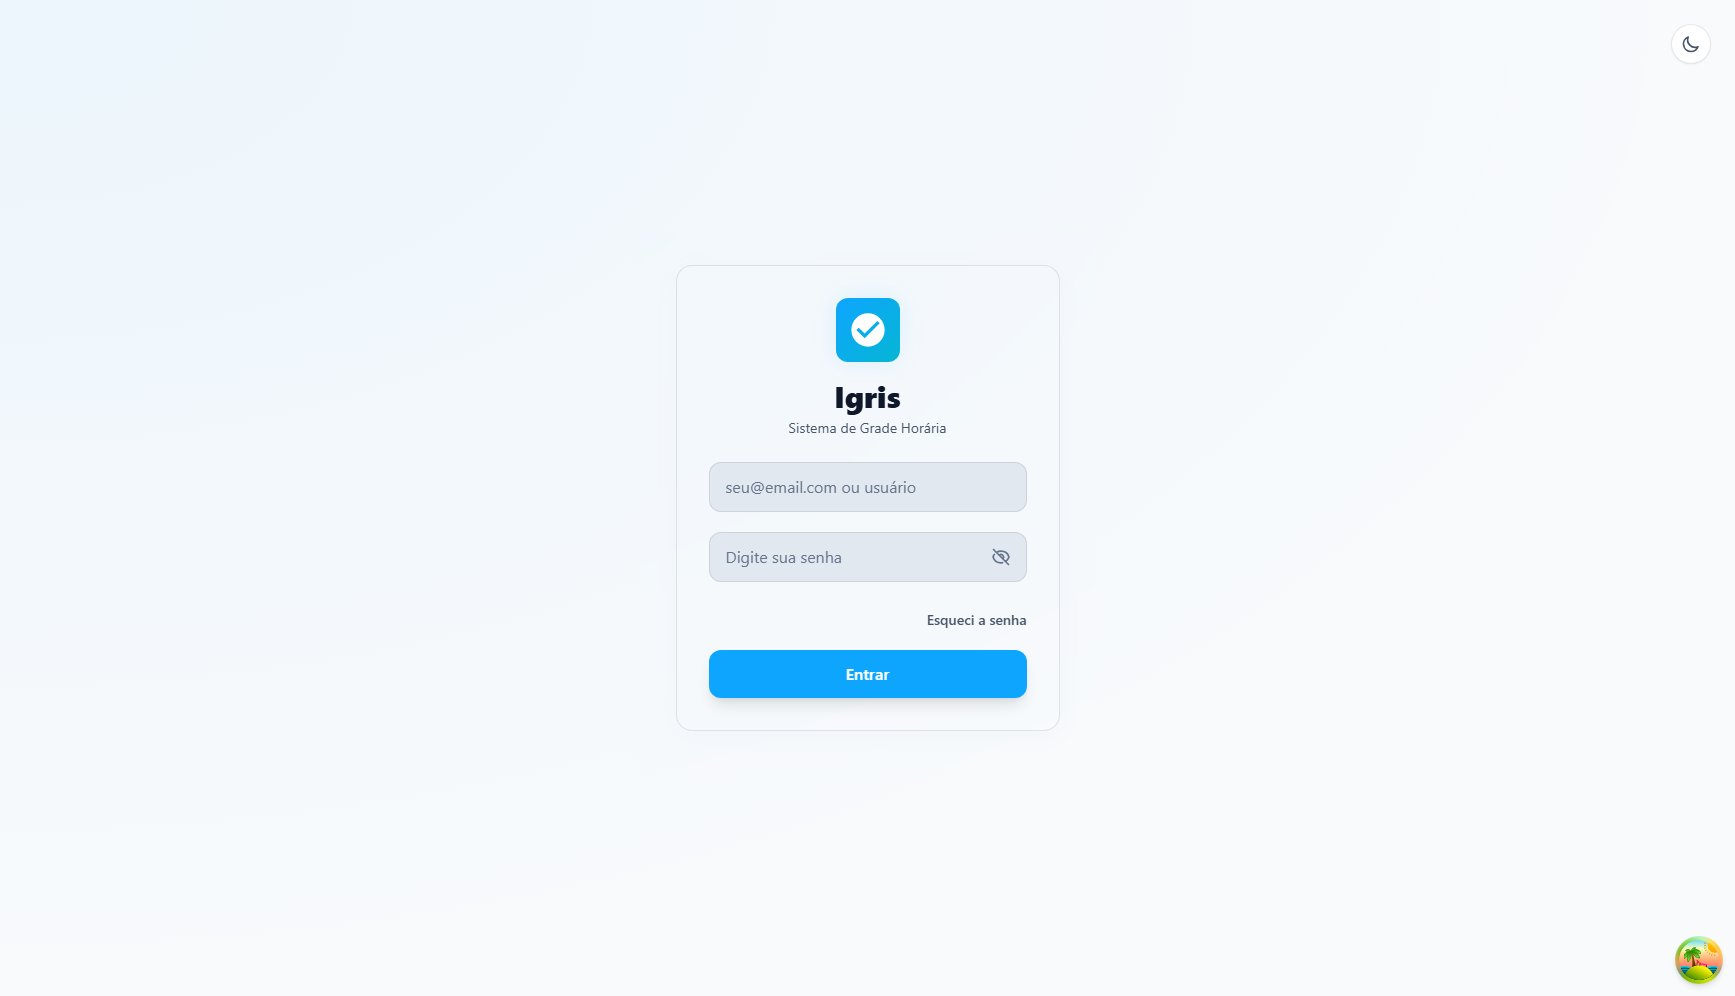
\includegraphics[width=\textwidth]{figuras/paginas/Figura_18_PG1.jpg}
\fonteautores
\end{figure}

A tela de login é o ponto inicial de interação do usuário com o sistema IGRIS. O usuário encontra um formulário composto pelos campos para inserção de e-mail (ou nome de usuário) e senha. A tela também oferece um botão para exibir ou ocultar a senha, a função "Esqueci a senha" e o botão "Entrar" para acessar o sistema. O design em tema escuro com detalhes em azul destaca a modernidade da aplicação.

\begin{longtable}{|L{4.1cm}|L{5.2cm}|L{5.2cm}|}
\caption{Interações da Tela de Login}
\label{tab:interacoes-login} \\
\hline
\textbf{Comando} & \textbf{Ação} & \textbf{Observações} \\
\hline
\endfirsthead
\hline
\textbf{Comando} & \textbf{Ação} & \textbf{Observações} \\
\hline
\endhead
Informar e-mail ou nome de usuário & O sistema registra o identificador digitado para utilizá-lo na autenticação. & O campo é obrigatório e deve corresponder a um usuário previamente cadastrado. \\
\hline
Informar a senha & O sistema mantém o valor digitado oculto e o associa à tentativa de autenticação. & O preenchimento é obrigatório; por segurança, os caracteres são inicialmente representados por pontos. \\
\hline
Clicar no ícone de exibir ou ocultar senha & O sistema alterna a visualização dos caracteres da senha, sem modificar o valor informado. & A função permite conferir a digitação e não interfere nas credenciais enviadas. \\
\hline
Clicar em ``Entrar'' com os campos vazios & O sistema impede o envio do formulário e indica os campos que precisam ser preenchidos. & Deve ser apresentada uma mensagem de obrigatoriedade próxima aos respectivos campos. \\
\hline
Clicar em ``Entrar'' com credenciais inválidas & O sistema rejeita a autenticação e mantém o usuário na tela de login. & A mensagem de erro não deve revelar se o identificador ou a senha está incorreto, preservando a segurança da conta. \\
\hline
Clicar em ``Entrar'' com credenciais válidas & O sistema valida os dados, gera o token de acesso e redireciona o usuário ao ambiente correspondente. & Caso existam múltiplos perfis associados à conta, o usuário deve ser direcionado à tela de seleção de perfil. \\
\hline
Clicar em ``Esqueci a senha'' & O sistema abre a tela de recuperação de senha. & O fluxo seguinte solicita o e-mail associado à conta para o envio do link de recuperação. \\
\hline
Clicar no ícone de alteração de tema & O sistema alterna a aparência da interface entre os temas claro e escuro. & A mudança é apenas visual e não altera os dados preenchidos nem o processo de autenticação. \\
\hline
\end{longtable}

\fonteautores

% PG2.jpg
\begin{figure}[H]
\centering
\caption{Tela de Recuperação de Senha}
\label{fig:PG2}
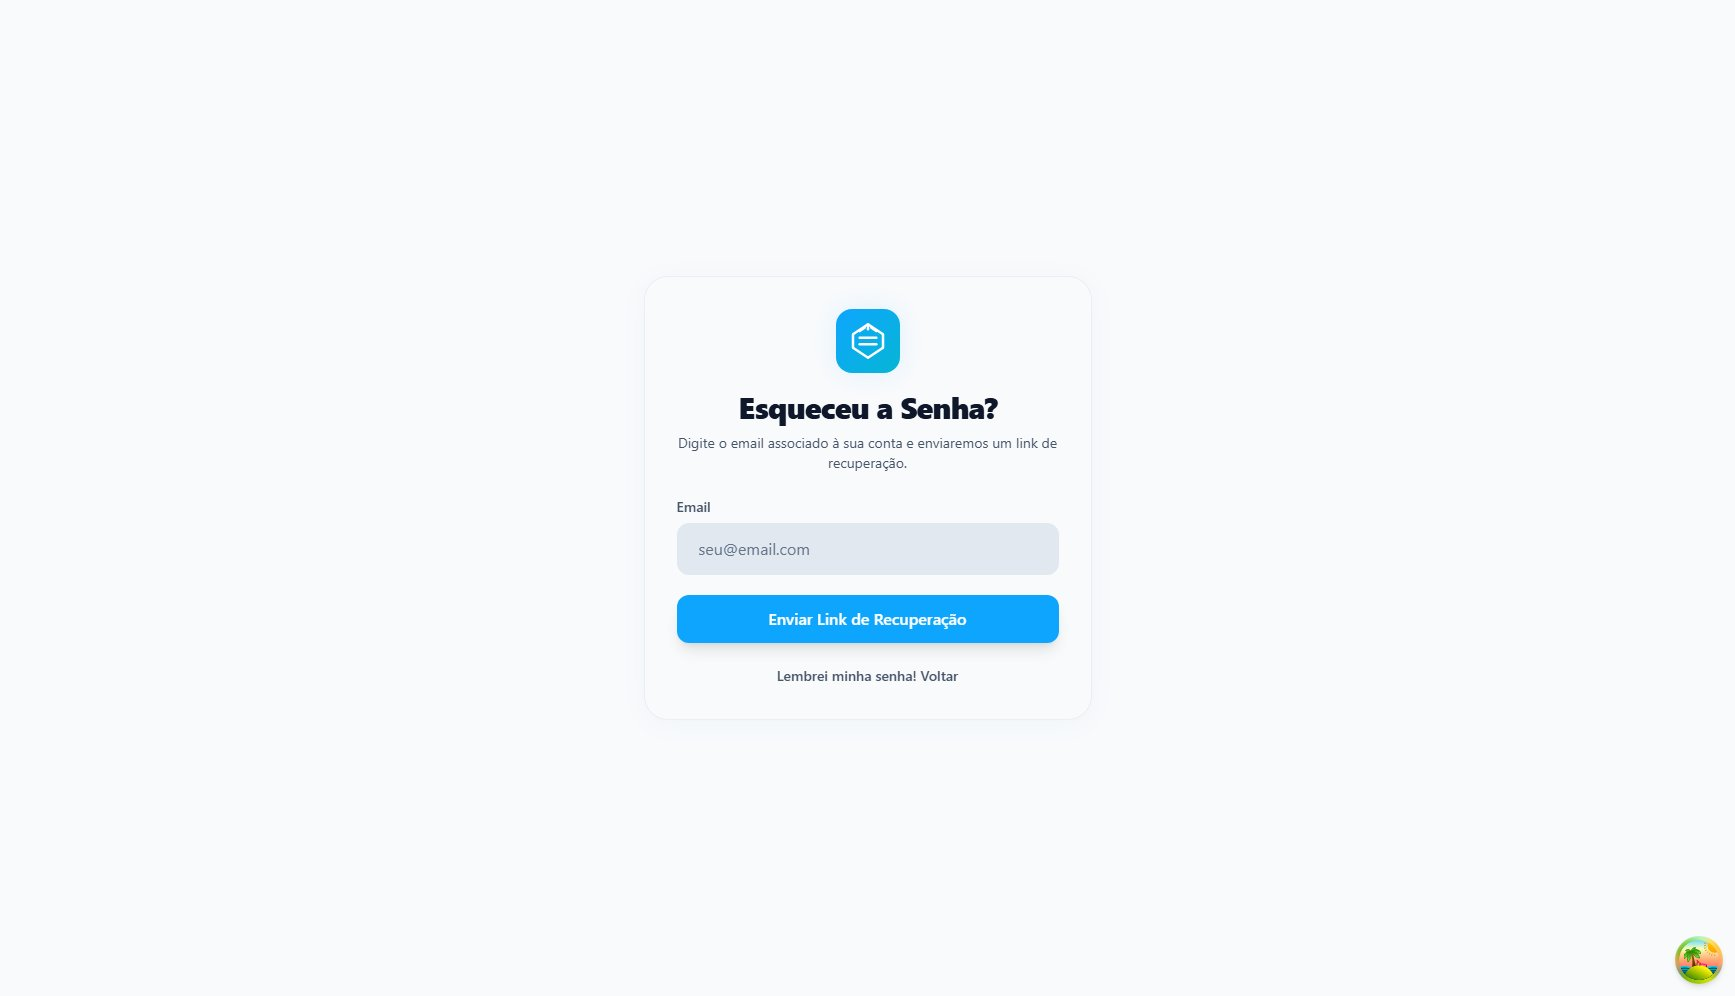
\includegraphics[width=\textwidth]{figuras/paginas/Figura_19_PG2.jpg}
\fonteautores
\end{figure}

A tela de recuperação de senha é acessada pelo link "Esqueci a senha". Nela, o usuário é instruído a digitar o e-mail associado à sua conta para que o sistema envie um link de recuperação. A interface simples e focada fornece os botões "Enviar Link de Recuperação" e um atalho para voltar à tela de login.

\begin{tabelainteracoes}{Interações da Tela de Recuperação de Senha}{tab:interacoes-recuperacao-senha}
Informar o e-mail da conta & O sistema registra o endereço para localizar o cadastro e preparar a solicitação de recuperação. & O campo é obrigatório e deve possuir formato de e-mail válido. \\
\hline
Clicar em ``Enviar Link de Recuperação'' com o campo vazio ou inválido & O sistema não envia a solicitação e informa que o e-mail precisa ser corrigido. & A validação deve ocorrer antes da comunicação com o serviço de recuperação. \\
\hline
Clicar em ``Enviar Link de Recuperação'' com um e-mail válido & O sistema gera um token temporário e envia ao endereço informado as instruções para definição de uma nova senha. & Por segurança, a confirmação não deve revelar se o e-mail está ou não cadastrado. O link deve possuir prazo de validade e uso único. \\
\hline
Clicar em ``Lembrei minha senha! Voltar'' & O sistema encerra o fluxo de recuperação e retorna à tela de login. & Nenhuma solicitação é criada e o e-mail digitado pode ser descartado. \\
\hline
Utilizar um link expirado ou já usado & O sistema recusa a redefinição e orienta o usuário a solicitar um novo link. & O token de recuperação deve ser validado antes de permitir a alteração da senha. \\
\hline
\end{tabelainteracoes}

% PG3.jpg
\begin{figure}[H]
\centering
\caption{Tela de Seleção de Perfil}
\label{fig:PG3}
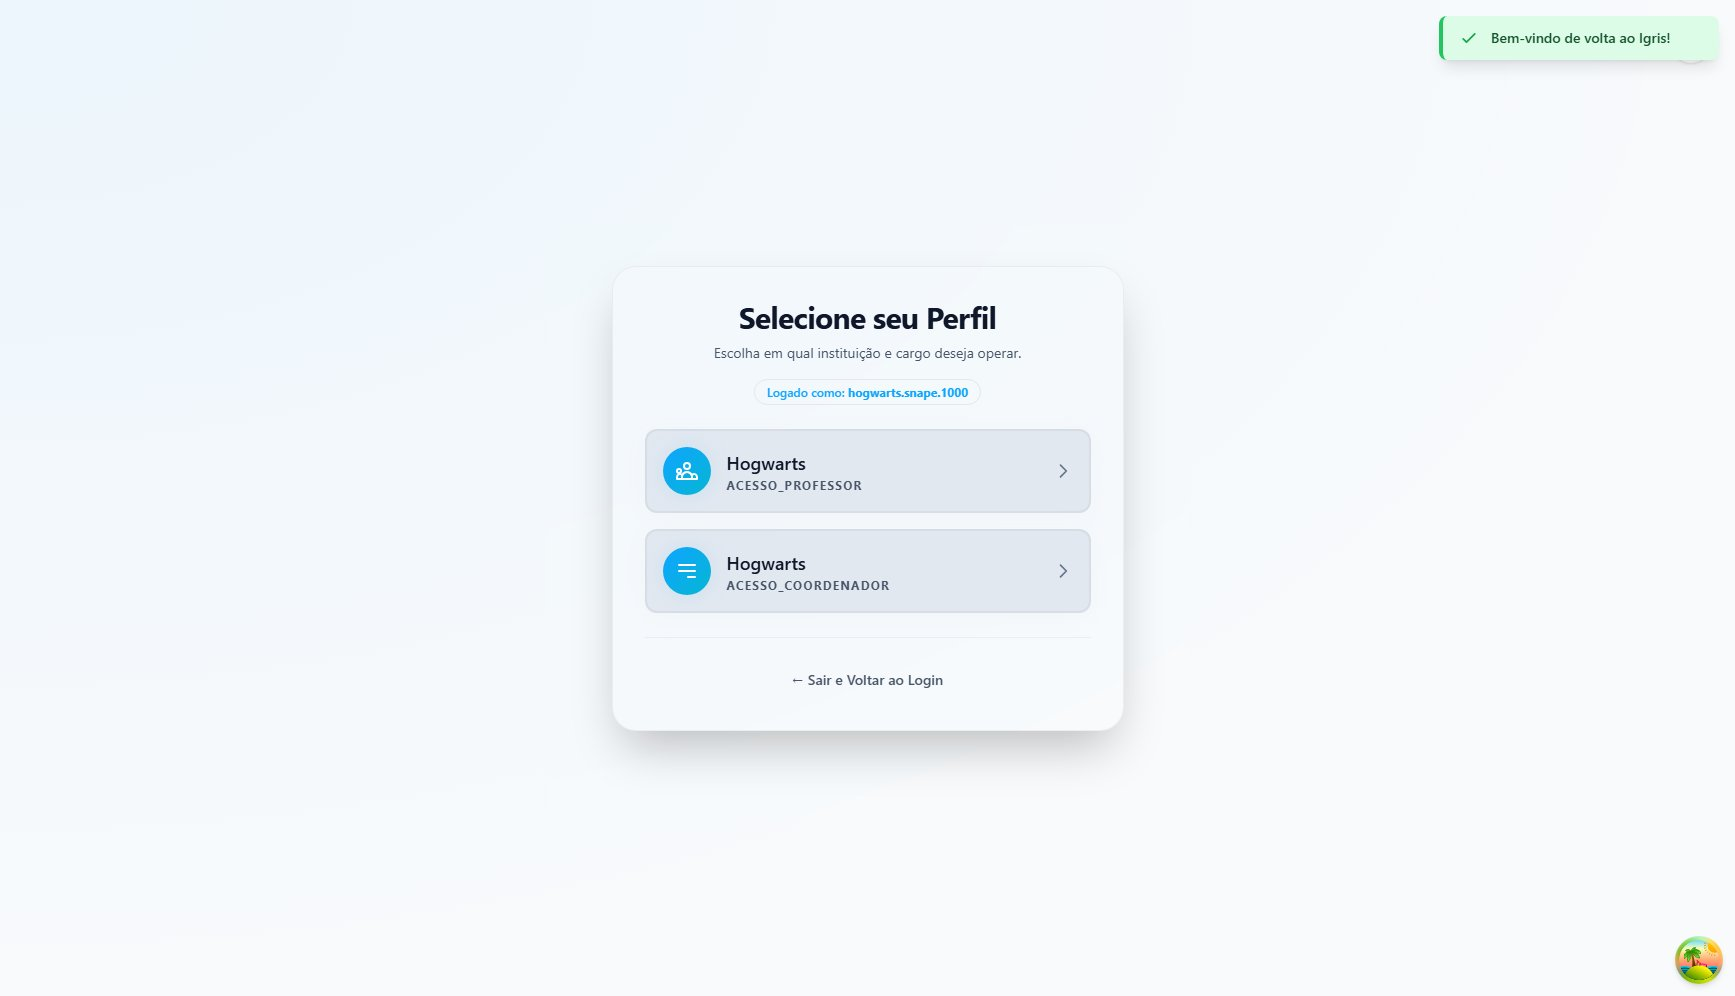
\includegraphics[width=\textwidth]{figuras/paginas/Figura_20_PG3.jpg}
\fonteautores
\end{figure}

Após a autenticação, se o usuário possuir mais de um papel, é apresentada a tela de seleção de perfil. Essa interface exibe as instituições e cargos disponíveis, como \texttt{ACESSO\_\allowbreak COORDENADOR} e \texttt{ACESSO\_\allowbreak PROFESSOR}, permitindo que o usuário direcione sua navegação ao ambiente adequado. Também há uma opção para sair e voltar ao login.

\begin{tabelainteracoes}{Interações da Tela de Seleção de Perfil}{tab:interacoes-selecao-perfil}
Visualizar os perfis disponíveis & O sistema lista somente os perfis e instituições vinculados à conta autenticada. & Cada opção deve identificar o contexto institucional e o nível de acesso correspondente. \\
\hline
Clicar em um perfil & O sistema ativa o contexto selecionado, emite um novo token de acesso e direciona o usuário ao painel adequado. & As permissões e funcionalidades exibidas passam a respeitar o perfil escolhido. \\
\hline
Selecionar um perfil sem vínculo válido ou inativo & O sistema impede o acesso e informa que o perfil não está disponível. & O vínculo deve ser validado novamente no servidor, mesmo que apareça previamente na interface. \\
\hline
Clicar em ``Sair e Voltar ao Login'' & O sistema encerra a sessão atual e apresenta novamente a tela de autenticação. & Tokens e dados temporários da sessão devem ser invalidados. \\
\hline
\end{tabelainteracoes}

% PG4.jpg
\begin{figure}[H]
\centering
\caption{Painel do Coordenador - Visão Geral}
\label{fig:PG4}
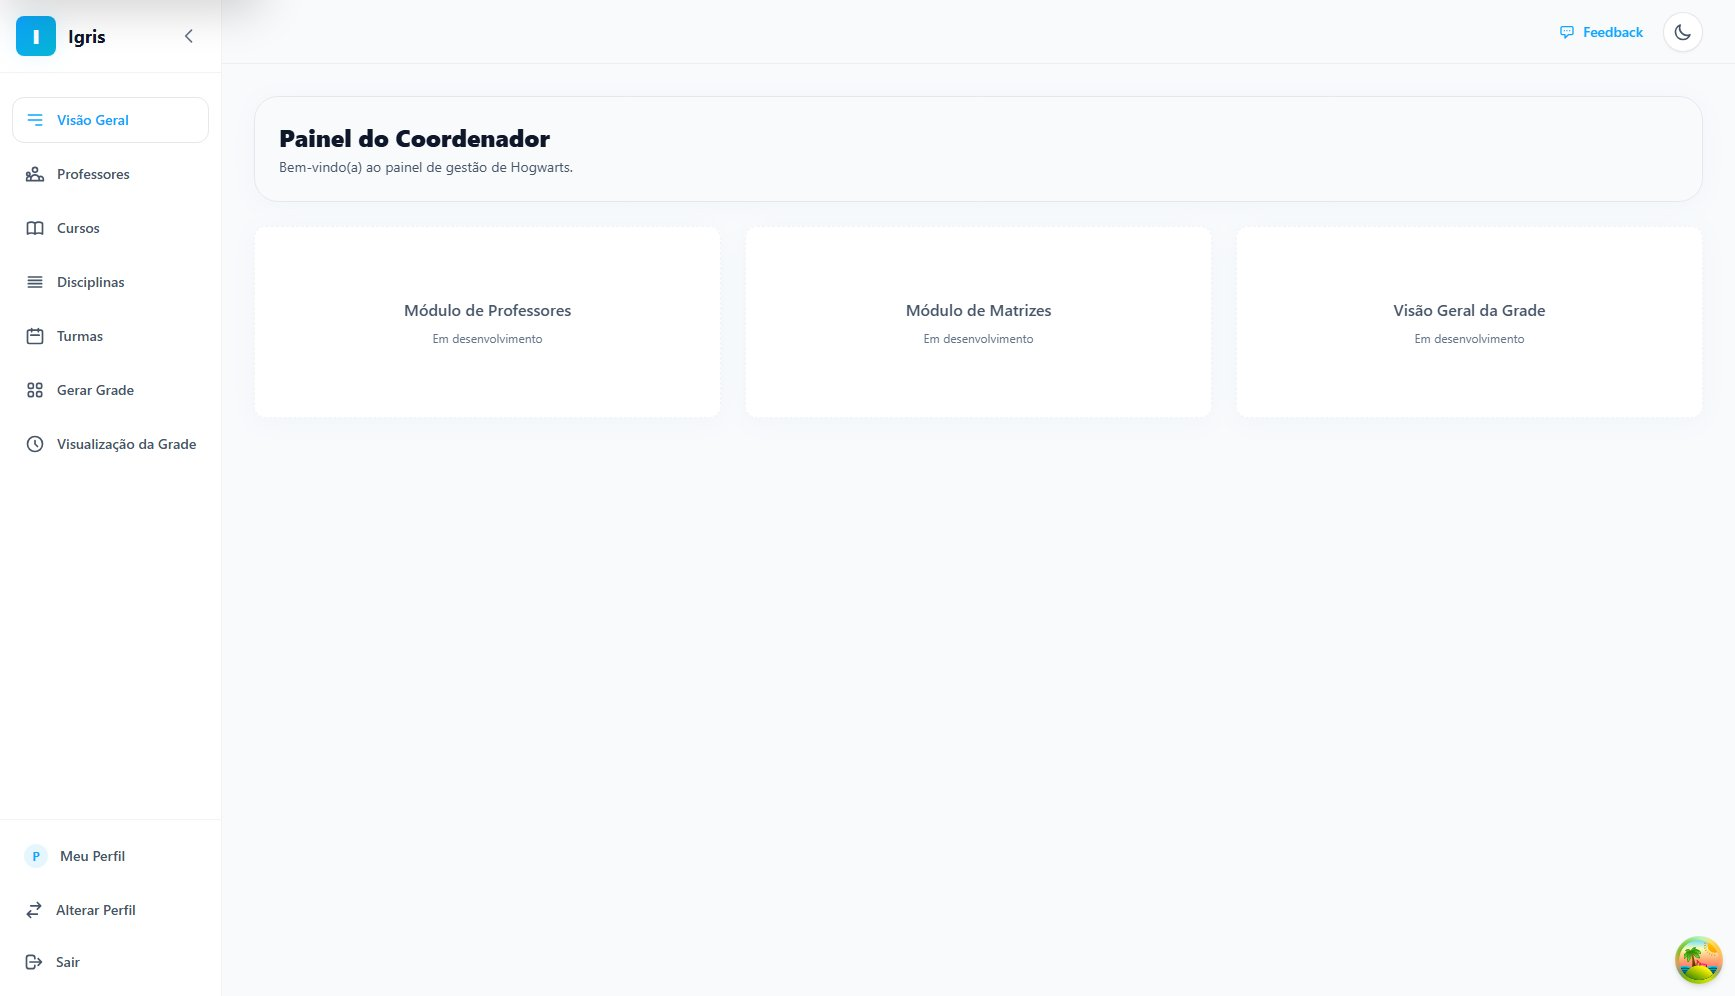
\includegraphics[width=\textwidth]{figuras/paginas/Figura_21_PG4.jpg}
\fonteautores
\end{figure}

O Painel do Coordenador apresenta a interface principal do gestor acadêmico. Um menu lateral à esquerda fornece acesso rápido às seções essenciais do sistema: Professores, Cursos, Disciplinas, Turmas, Gerar Grade e Visualização da Grade, centralizando o controle da grade horária da instituição.

\begin{tabelainteracoes}{Interações do Painel do Coordenador}{tab:interacoes-painel-coordenador}
Clicar em uma opção do menu lateral & O sistema abre o módulo correspondente e destaca a seção ativa. & Apenas módulos autorizados para o perfil de coordenador devem permanecer disponíveis. \\
\hline
Clicar em um cartão de acesso rápido & O sistema direciona o usuário ao módulo indicado, como Professores, Matrizes ou Visualização da Grade. & O cartão funciona como atalho e deve produzir o mesmo resultado da opção equivalente no menu. \\
\hline
Clicar em ``Meu Perfil'' & O sistema abre as informações e configurações da conta do usuário. & Alterações pessoais não devem modificar automaticamente o perfil institucional ativo. \\
\hline
Clicar em ``Alterar Perfil'' & O sistema retorna à seleção de perfil para que outro vínculo seja ativado. & Ao confirmar a troca, as permissões e o contexto institucional devem ser recarregados. \\
\hline
Clicar em ``Sair'' & O sistema encerra a sessão e retorna à tela de login. & O token de acesso deve ser invalidado ou removido do cliente. \\
\hline
\end{tabelainteracoes}

% PG5.jpg
\begin{figure}[H]
\centering
\caption{Tela de Gerenciamento de Corpo Docente}
\label{fig:PG5}
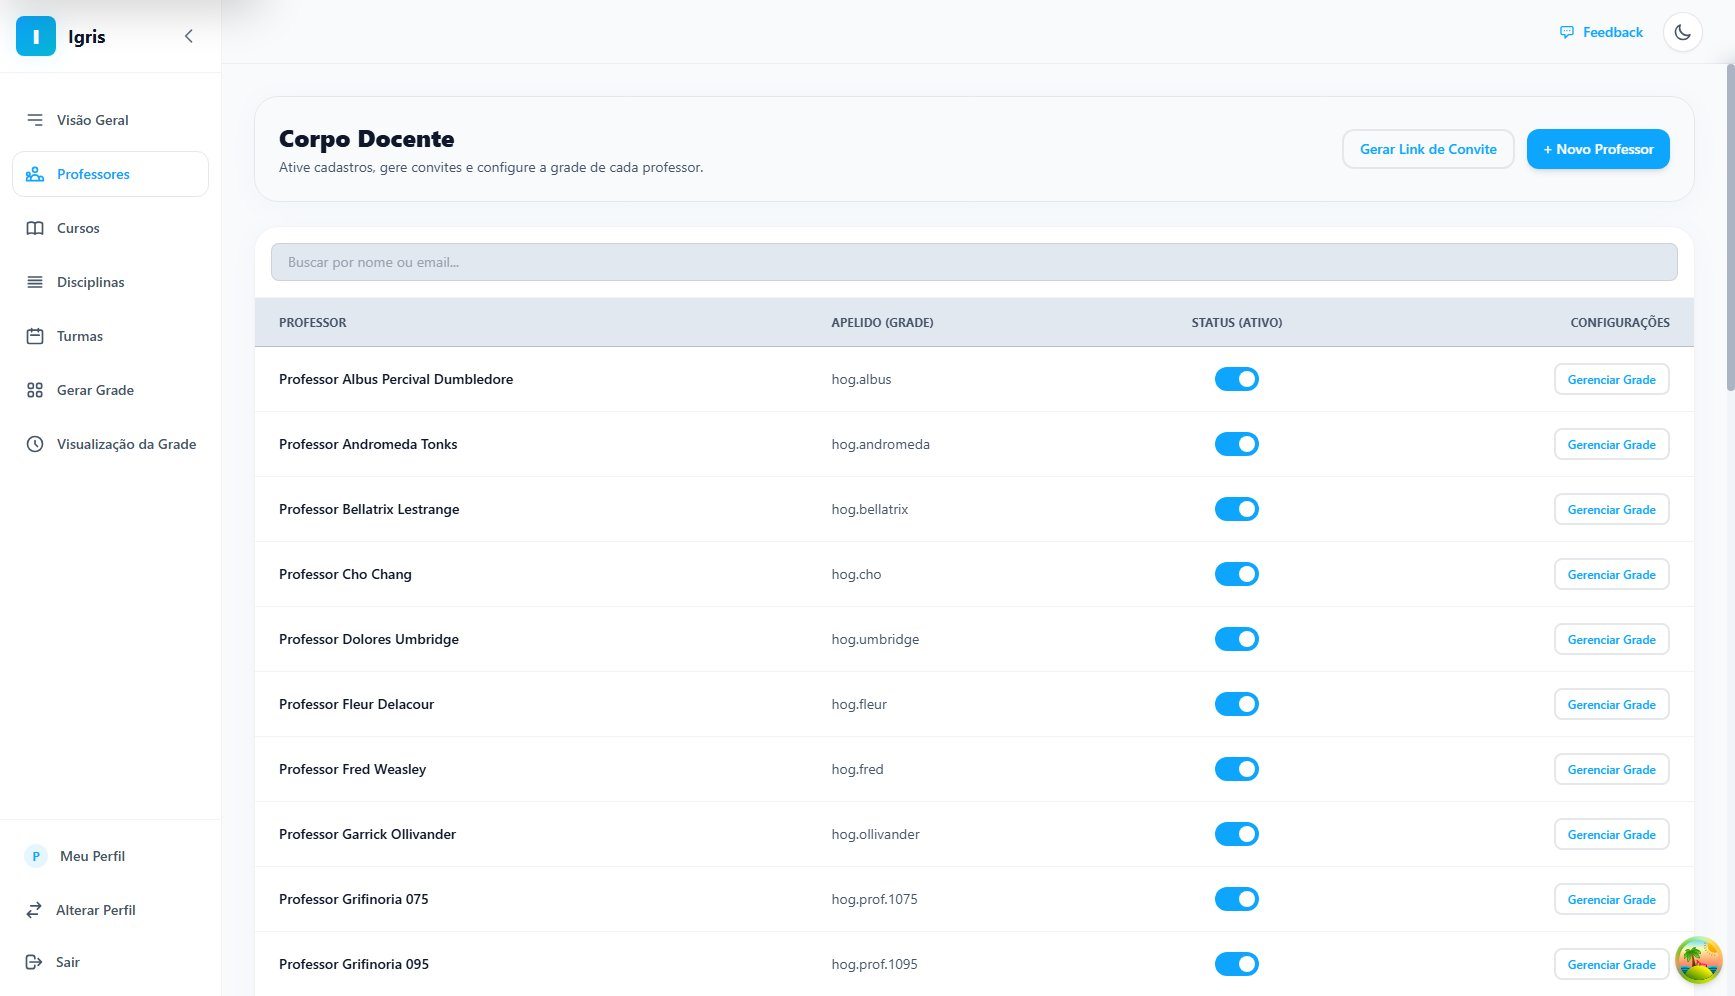
\includegraphics[width=\textwidth]{figuras/paginas/Figura_22_PG5.jpg}
\fonteautores
\end{figure}

Na tela de professores, o coordenador pode visualizar e gerenciar o corpo docente. O sistema apresenta uma lista com o nome, e-mail/login e status de cada professor. Interruptores de ativação (toggles) permitem habilitar ou desabilitar o acesso dos docentes ao sistema rapidamente, além de oferecer botões para gerenciar a grade individual de cada um.

\begin{tabelainteracoes}{Interações da Tela de Gerenciamento de Corpo Docente}{tab:interacoes-corpo-docente}
Pesquisar pelo nome ou e-mail do professor & O sistema filtra a listagem conforme o texto informado. & Quando não houver correspondências, deve ser exibida uma indicação de lista vazia. \\
\hline
Alterar o interruptor de status & O sistema ativa ou desativa o acesso do professor e atualiza o estado apresentado na lista. & A desativação impede novos acessos, mas não deve excluir o cadastro nem os vínculos acadêmicos existentes. \\
\hline
Clicar em ``Gerenciar Grade'' & O sistema abre as configurações de áreas de atuação e disponibilidade do professor selecionado. & As alterações devem afetar somente o docente correspondente à linha acionada. \\
\hline
Clicar em ``Gerar Link de Convite'' & O sistema cria um convite seguro para o autocadastro de um novo professor. & O link deve possuir token único, prazo de validade e associação com a instituição. \\
\hline
Clicar em ``Novo Professor'' & O sistema abre o formulário de cadastro manual de docente. & Somente usuários autorizados podem criar ou ativar professores. \\
\hline
\end{tabelainteracoes}

% PG6.jpg
\begin{figure}[H]
\centering
\caption{Geração de Link de Convite para Docentes}
\label{fig:PG6}
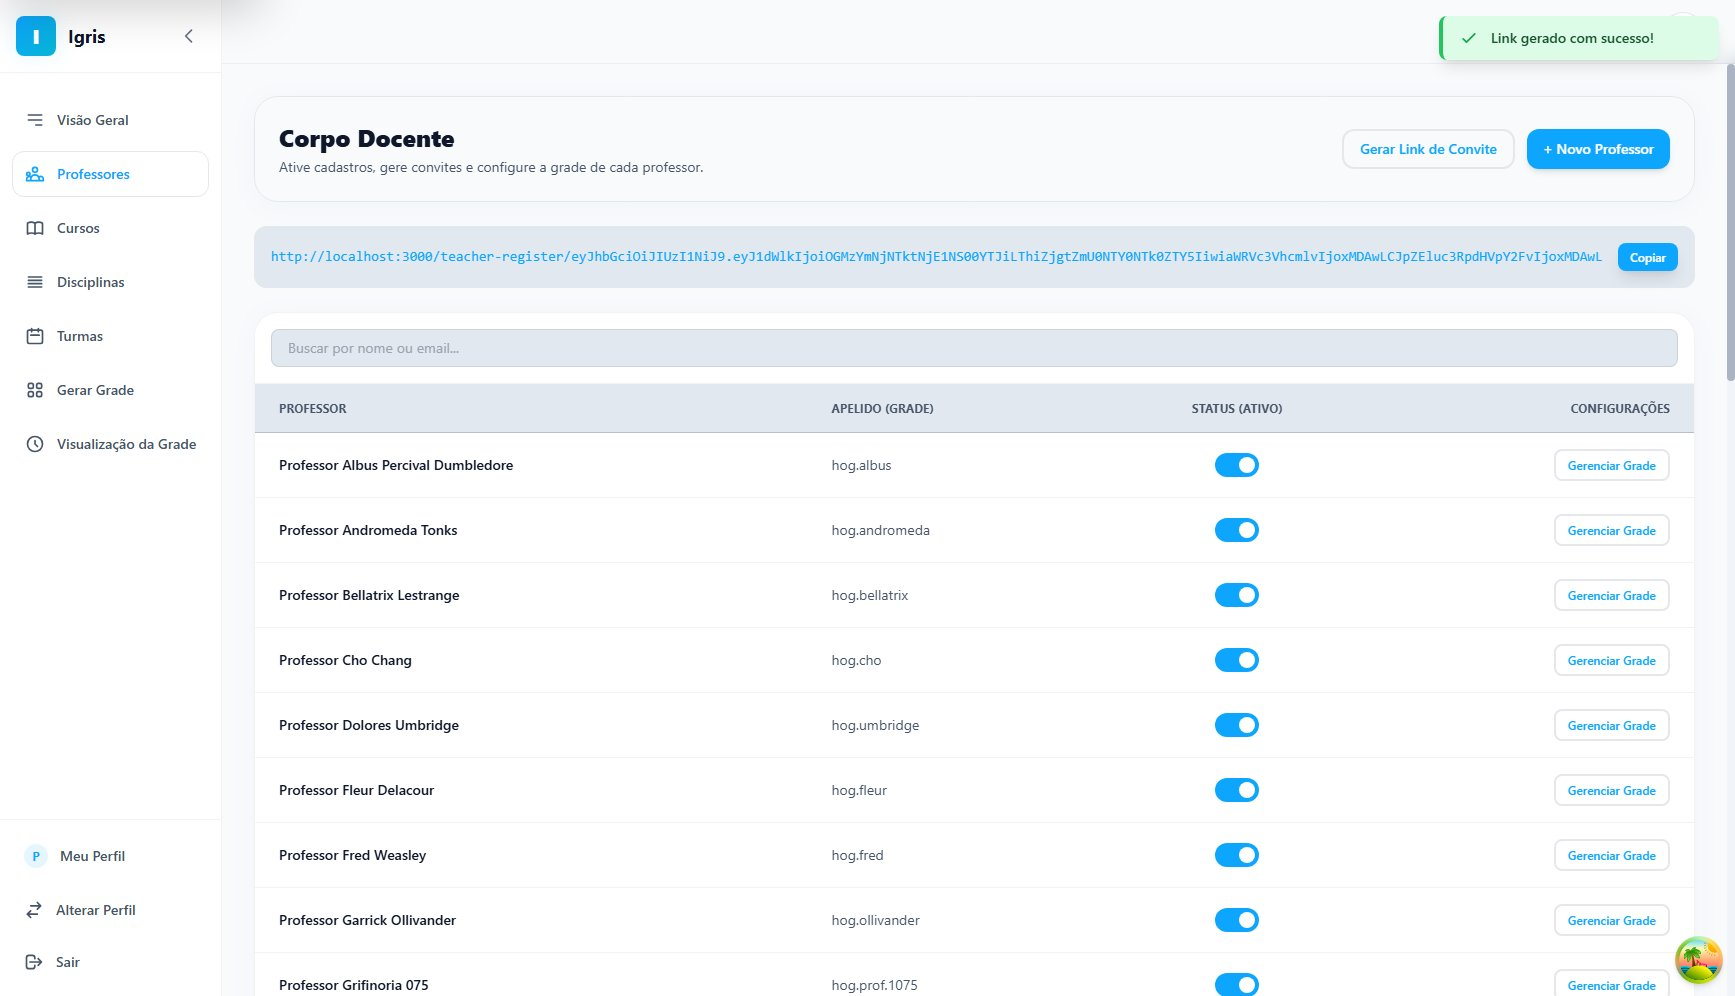
\includegraphics[width=\textwidth]{figuras/paginas/Figura_23_PG6.jpg}
\fonteautores
\end{figure}

A tela do corpo docente também permite a geração de um link de convite. Ao clicar no botão correspondente, o sistema cria e exibe uma URL específica que pode ser copiada e compartilhada com os professores, facilitando o auto-cadastramento deles na plataforma institucional.

\begin{tabelainteracoes}{Interações da Geração de Link de Convite}{tab:interacoes-link-convite-docente}
Clicar em ``Gerar Link de Convite'' & O sistema cria um token seguro e apresenta a URL de cadastro na própria tela. & O convite deve estar vinculado à instituição e ao perfil de professor. \\
\hline
Clicar em ``Copiar'' & O sistema envia a URL exibida para a área de transferência e confirma a operação. & A cópia não altera a validade nem permite a reutilização de um convite já consumido. \\
\hline
Compartilhar e acessar o link válido & O sistema abre o formulário de autocadastro e associa o novo usuário ao contexto do convite. & Após a conclusão do cadastro, o token deve expirar para impedir novos usos. \\
\hline
Acessar um convite inválido ou expirado & O sistema bloqueia o cadastro e informa que um novo convite deve ser solicitado. & Nenhum perfil ou vínculo institucional deve ser criado nessa situação. \\
\hline
Solicitar a geração de outro link & O sistema cria uma nova URL, independente da anterior. & Conforme a regra adotada, o convite anterior pode ser invalidado para reduzir o risco de uso indevido. \\
\hline
\end{tabelainteracoes}

% PG7.jpg
\begin{figure}[H]
\centering
\caption{Tela de Cadastro de Novo Professor}
\label{fig:PG7}
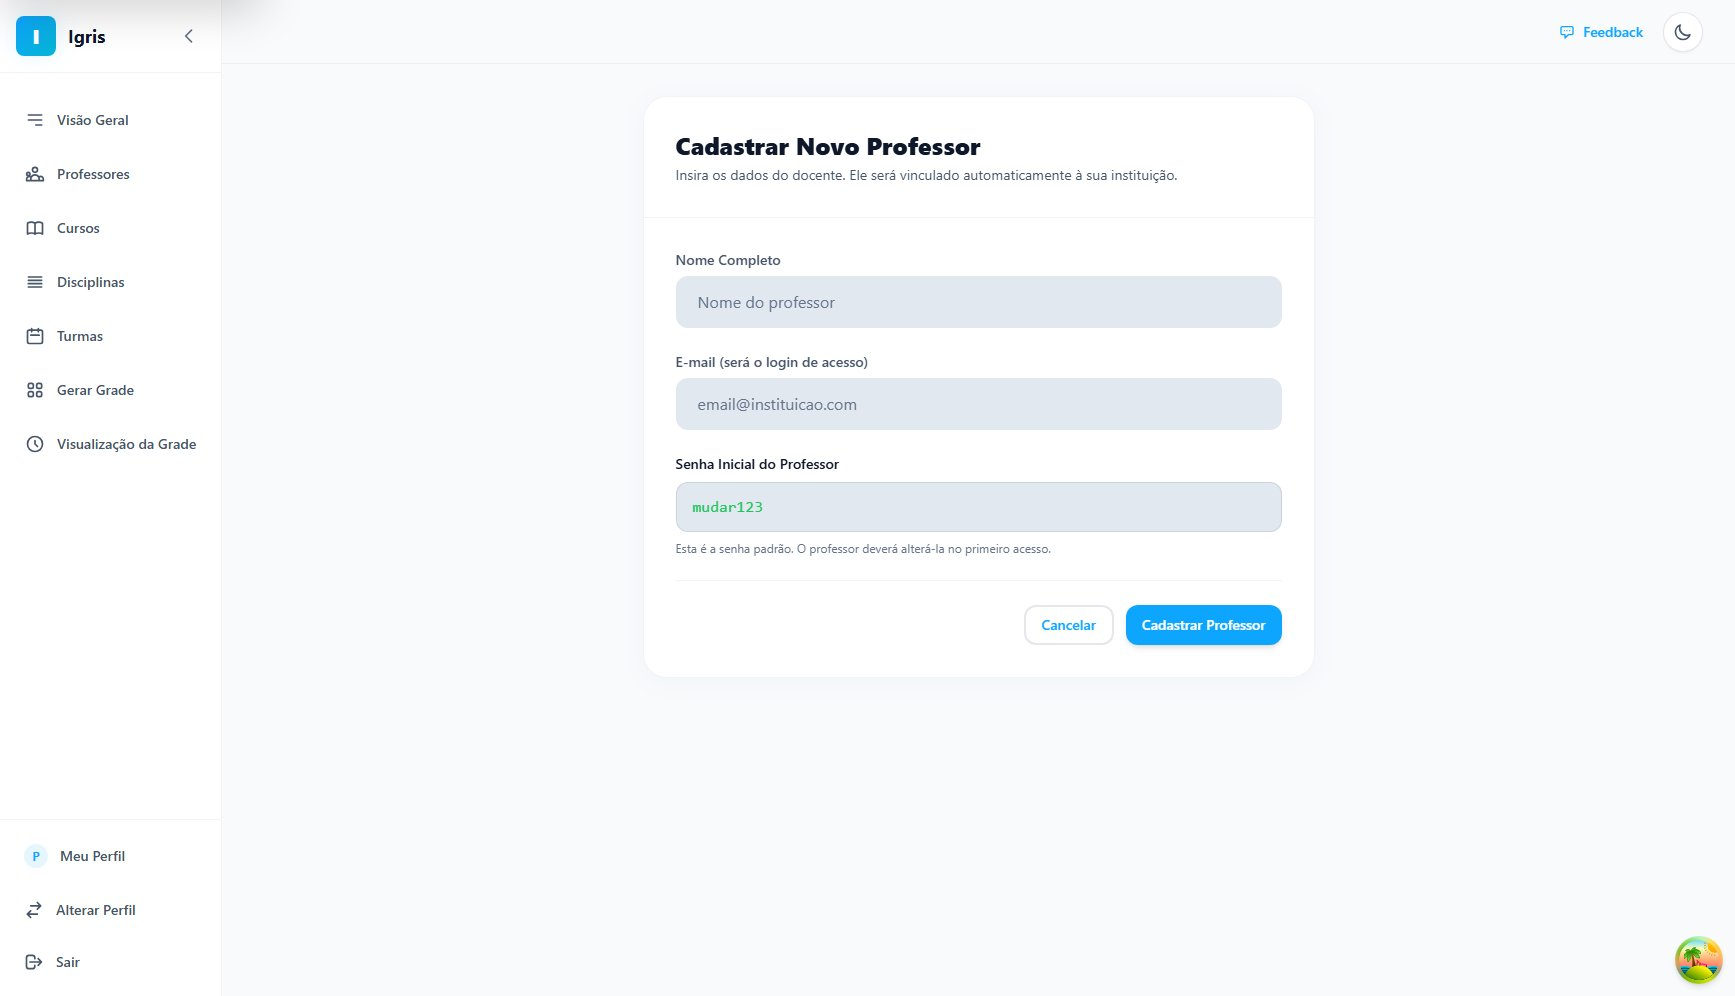
\includegraphics[width=\textwidth]{figuras/paginas/Figura_24_PG7.jpg}
\fonteautores
\end{figure}

Acessada pelo botão "Novo Professor", esta janela em formato de sobreposição (modal) permite o cadastro manual de um docente. O coordenador insere o nome, e-mail e uma senha inicial padrão que o professor deverá alterar posteriormente em seu primeiro acesso.

\begin{tabelainteracoes}{Interações da Tela de Cadastro de Novo Professor}{tab:interacoes-cadastro-professor}
Informar o nome completo & O sistema registra o nome que identificará o docente nas listagens e grades. & O campo é obrigatório e não deve aceitar apenas espaços em branco. \\
\hline
Informar o e-mail ou login & O sistema utiliza o valor como identificador de acesso do professor. & O endereço deve possuir formato válido e não pode estar associado a outro usuário. \\
\hline
Informar a senha inicial & O sistema oculta os caracteres e prepara a senha para armazenamento seguro. & Devem ser aplicadas as regras mínimas de segurança; a senha precisa ser criptografada e alterada no primeiro acesso. \\
\hline
Clicar em ``Cadastrar Professor'' com dados válidos & O sistema cria o usuário, vincula o perfil de professor e fecha o formulário. & A listagem deve ser atualizada e uma mensagem de sucesso apresentada. \\
\hline
Clicar em ``Cadastrar Professor'' com dados inválidos & O sistema mantém o formulário aberto e destaca os campos que precisam de correção. & O cadastro não pode ser criado parcialmente. \\
\hline
Clicar em ``Cancelar'' ou no ícone de fechar & O sistema fecha a janela sem salvar o novo professor. & Se houver dados preenchidos, eles são descartados. \\
\hline
\end{tabelainteracoes}

% PG8.jpg
\begin{figure}[H]
\centering
\caption{Tela de Gerenciamento de Turmas}
\label{fig:PG8}
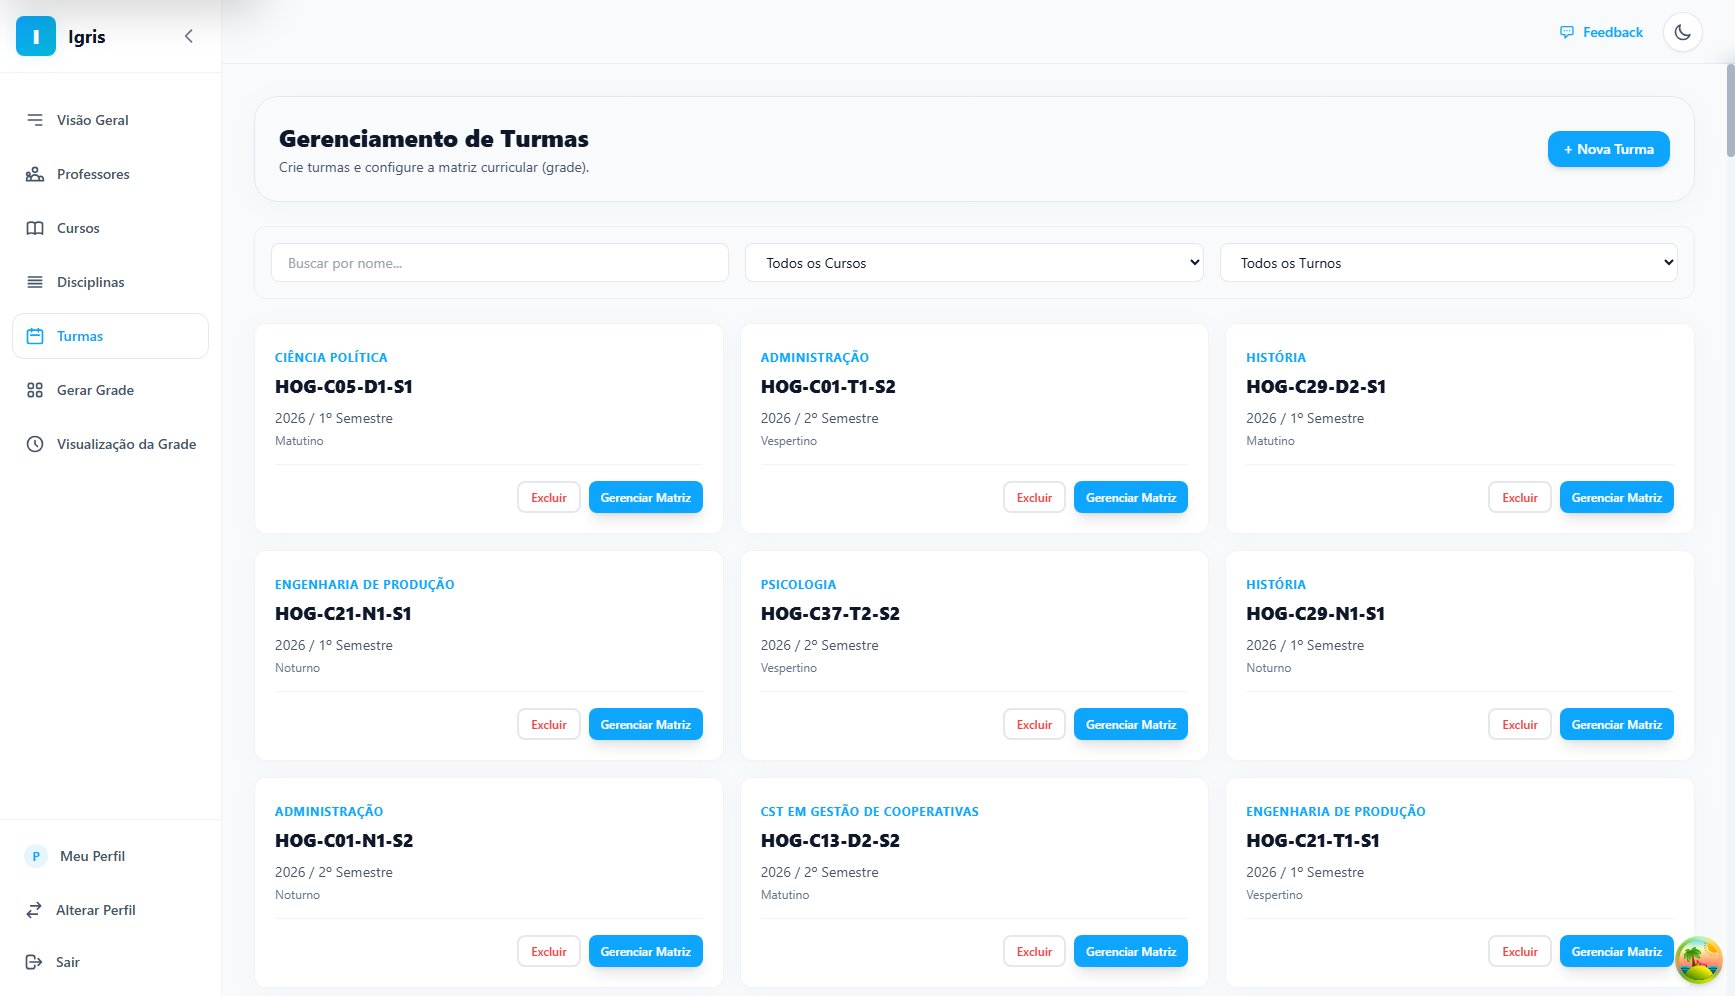
\includegraphics[width=\textwidth]{figuras/paginas/Figura_25_PG8.jpg}
\fonteautores
\end{figure}

A tela de Gerenciamento de Turmas apresenta todas as turmas cadastradas organizadas em cartões. O coordenador pode visualizar dados como curso associado, turno (matutino, vespertino, noturno) e período letivo. Estão disponíveis ferramentas de busca, filtros e botões para gerenciar a matriz de cada turma, além de uma opção para criar novas turmas.

\begin{tabelainteracoes}{Interações da Tela de Gerenciamento de Turmas}{tab:interacoes-gerenciamento-turmas}
Pesquisar uma turma pelo nome & O sistema filtra os cartões enquanto o usuário informa o termo de busca. & A busca deve considerar o identificador ou nome apresentado no cartão. \\
\hline
Selecionar os filtros de curso ou turno & O sistema restringe a listagem às turmas compatíveis com os critérios escolhidos. & Os filtros podem ser combinados e devem permitir o retorno à opção de exibir todos os registros. \\
\hline
Clicar em ``Gerenciar Matriz'' & O sistema abre a janela com os dados e as disciplinas vinculadas à turma selecionada. & A operação deve manter o contexto da turma acionada. \\
\hline
Clicar em ``Excluir'' & O sistema solicita confirmação e, se autorizado, remove a turma. & A exclusão deve ser bloqueada ou tratada quando existirem matrizes, grades ou alocações dependentes. \\
\hline
Clicar em ``Nova Turma'' & O sistema abre o formulário para criação de uma turma e de sua matriz inicial. & O novo registro deve ficar vinculado à coordenação ativa. \\
\hline
\end{tabelainteracoes}

% PG9.jpg
\begin{figure}[H]
\centering
\caption{Catálogo de Cursos}
\label{fig:PG9}
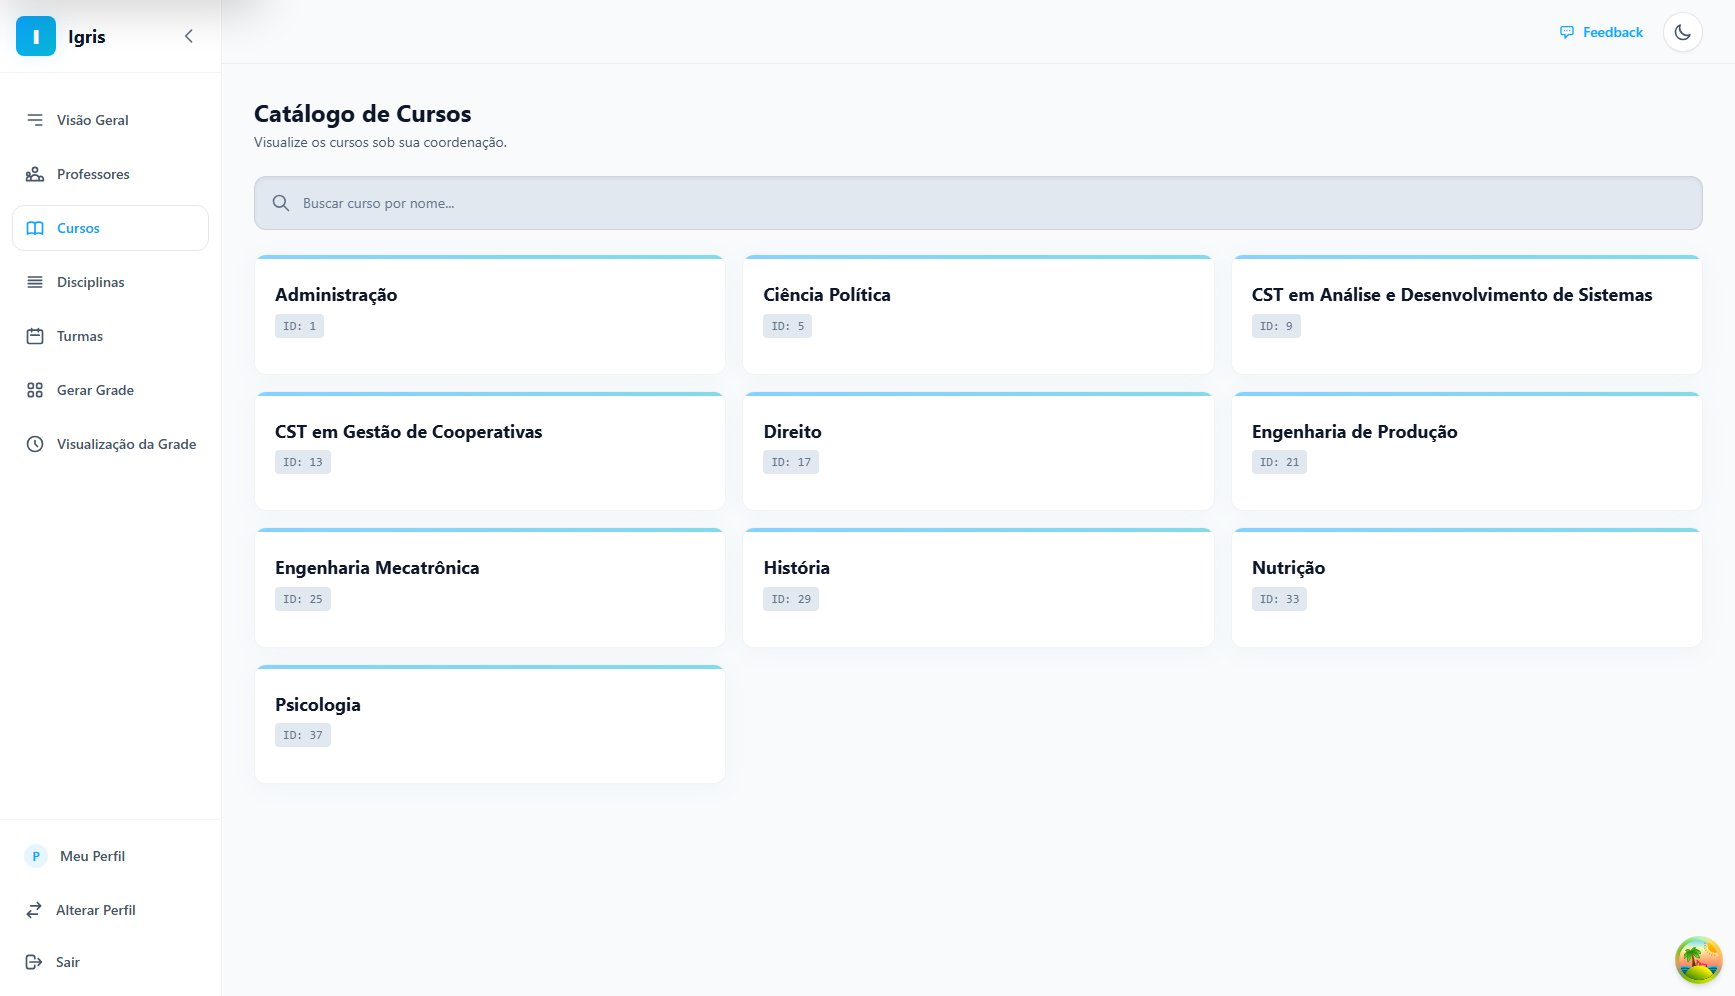
\includegraphics[width=\textwidth]{figuras/paginas/Figura_26_PG9.jpg}
\fonteautores
\end{figure}

A tela de cursos exibe as formações acadêmicas disponíveis sob a coordenação do usuário. Cada curso é representado por um cartão interativo contendo seu nome e identificador interno, fornecendo uma base estrutural para a criação de turmas e atribuição de disciplinas.

\begin{tabelainteracoes}{Interações do Catálogo de Cursos}{tab:interacoes-catalogo-cursos}
Pesquisar pelo nome do curso & O sistema filtra os cartões e exibe somente os cursos correspondentes. & A pesquisa deve aceitar correspondências parciais e informar quando nenhum resultado for encontrado. \\
\hline
Visualizar um cartão de curso & O sistema apresenta o nome e o identificador interno do registro. & Devem ser listados apenas os cursos pertencentes ao contexto institucional do coordenador. \\
\hline
Clicar em um cartão de curso & O sistema seleciona ou abre os detalhes do curso, conforme a operação disponível no módulo. & O curso serve de referência para turmas, matrizes e vínculos de disciplinas. \\
\hline
Tentar acessar um curso sem permissão & O sistema recusa a operação e mantém o usuário no catálogo autorizado. & A autorização deve ser verificada no servidor, e não apenas pela interface. \\
\hline
\end{tabelainteracoes}

% PG10.jpg
\begin{figure}[H]
\centering
\caption{Catálogo de Disciplinas}
\label{fig:PG10}
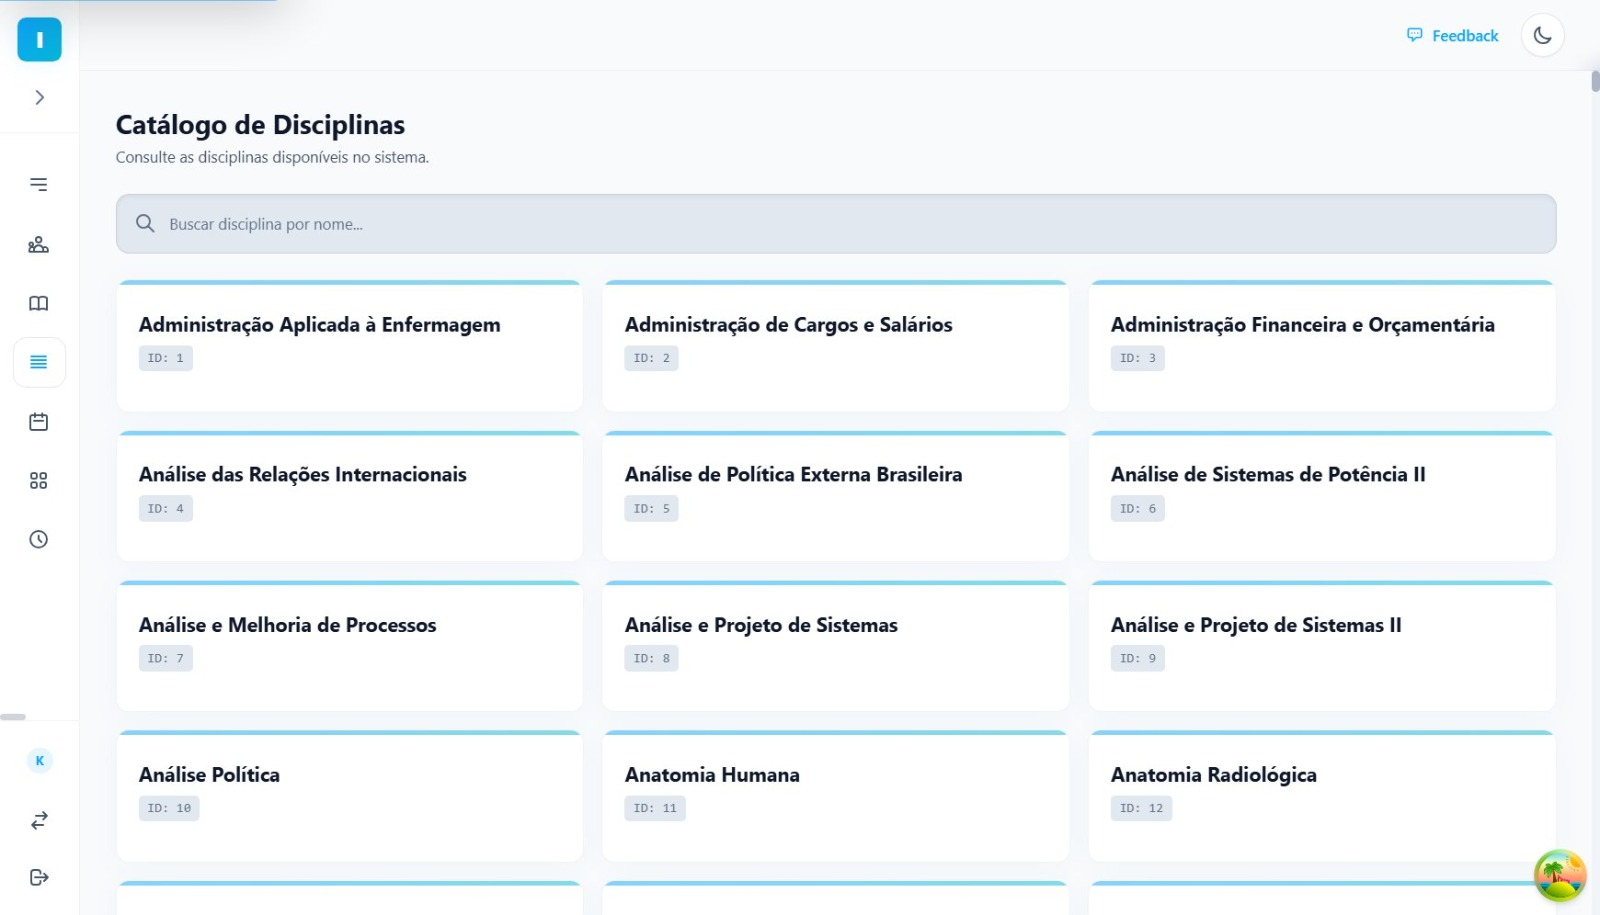
\includegraphics[width=\textwidth]{figuras/paginas/Figura_27_PG10.jpg}
\fonteautores
\end{figure}

No Catálogo de Disciplinas, o coordenador pode consultar todas as matérias que compõem o sistema. Uma barra de busca agiliza a localização de disciplinas específicas em meio aos diversos cartões que exibem o nome e ID de cada registro.

\begin{tabelainteracoes}{Interações do Catálogo de Disciplinas}{tab:interacoes-catalogo-disciplinas}
Pesquisar pelo nome da disciplina & O sistema filtra os cartões conforme o termo informado. & A pesquisa deve aceitar parte do nome e ignorar diferenças entre letras maiúsculas e minúsculas. \\
\hline
Limpar o campo de pesquisa & O sistema volta a apresentar todas as disciplinas disponíveis. & A listagem deve respeitar o contexto institucional e os filtros ativos. \\
\hline
Visualizar um cartão de disciplina & O sistema apresenta o nome e o identificador da matéria. & As informações são utilizadas posteriormente na composição de matrizes e áreas de atuação docente. \\
\hline
Clicar em uma disciplina & O sistema seleciona ou abre os detalhes do registro, quando essa ação estiver habilitada. & Alterações devem respeitar as permissões do perfil e preservar vínculos já utilizados em grades. \\
\hline
\end{tabelainteracoes}

% PG11.jpg
\begin{figure}[H]
\centering
\caption{Gerenciamento de Matriz da Turma}
\label{fig:PG11}
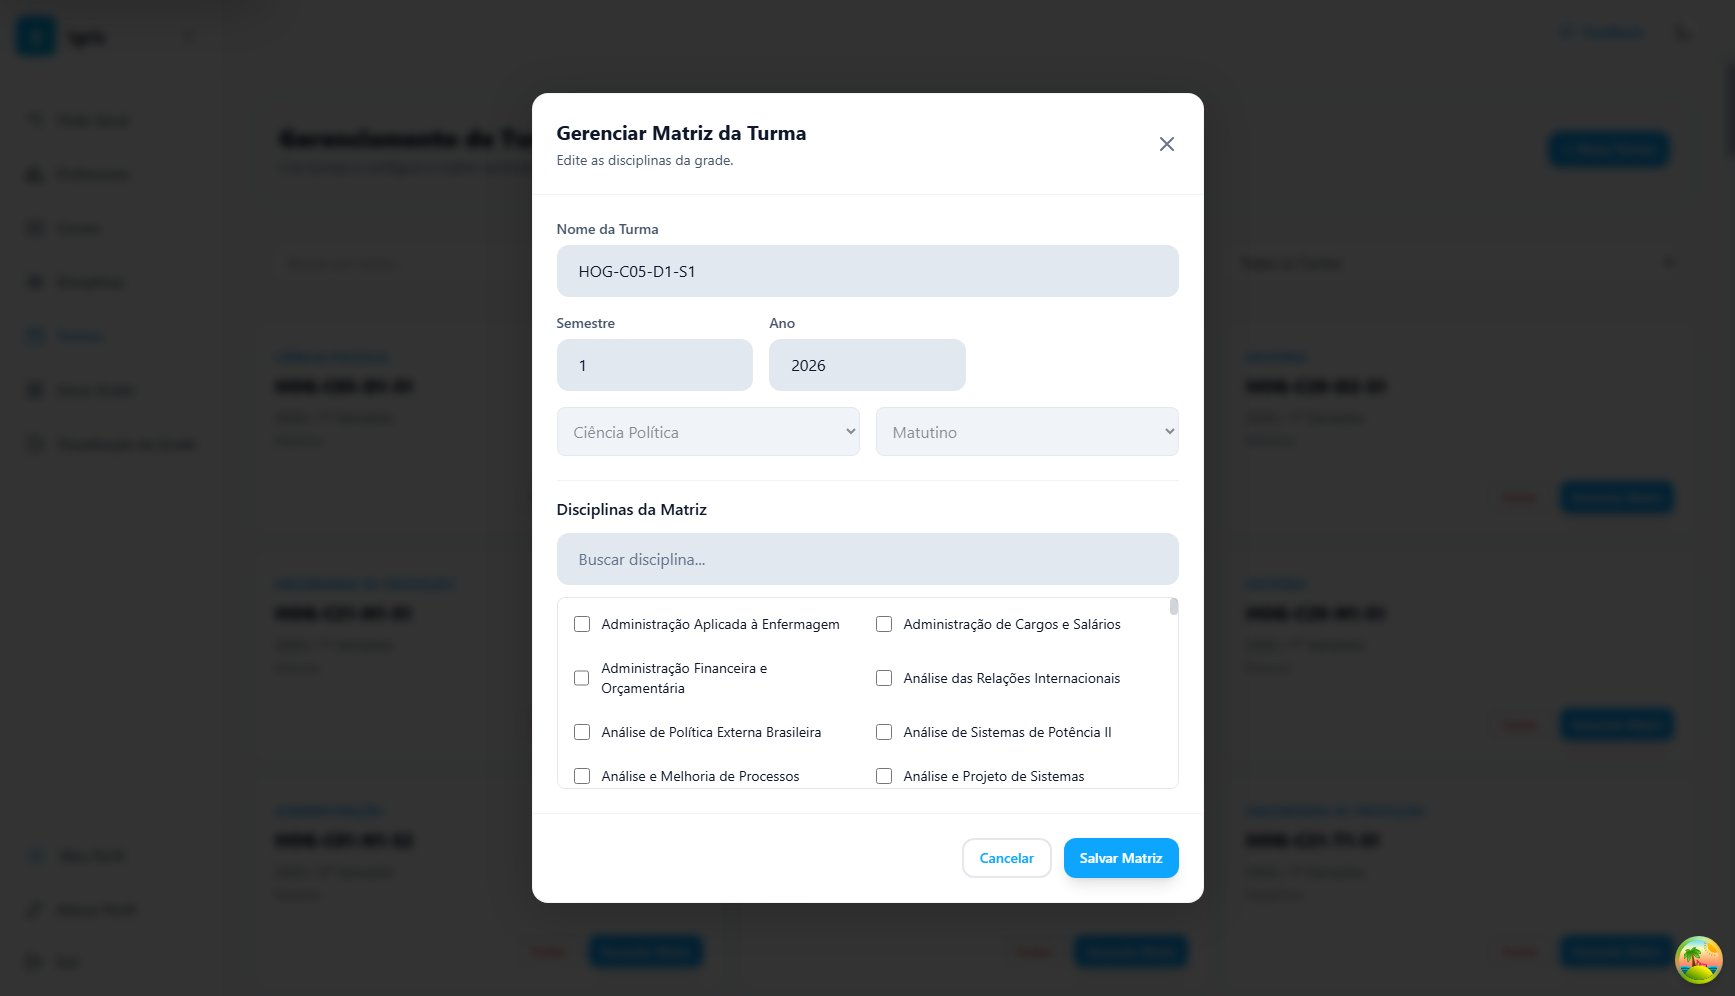
\includegraphics[width=\textwidth]{figuras/paginas/Figura_28_PG11.jpg}
\fonteautores
\end{figure}

Ao escolher gerenciar a matriz de uma turma, o sistema abre uma janela de edição. Nela, o coordenador visualiza os dados essenciais da turma em campos não editáveis e pode selecionar as disciplinas que farão parte da grade horária usando caixas de seleção, simplificando a montagem da matriz curricular.

\begin{tabelainteracoes}{Interações do Gerenciamento de Matriz da Turma}{tab:interacoes-matriz-turma}
Visualizar os dados da turma & O sistema apresenta nome, semestre, ano, curso e turno do registro selecionado. & Os campos contextuais permanecem bloqueados para evitar alterações acidentais durante a edição da matriz. \\
\hline
Pesquisar uma disciplina & O sistema filtra as opções disponíveis na lista da matriz. & A busca não modifica as seleções já realizadas. \\
\hline
Marcar ou desmarcar uma disciplina & O sistema inclui ou remove temporariamente a matéria da matriz da turma. & A mudança somente se torna definitiva após o salvamento. Disciplinas já alocadas podem exigir tratamento específico antes da remoção. \\
\hline
Clicar em ``Salvar Matriz'' & O sistema valida as seleções, atualiza os vínculos da matriz e fecha a janela. & Deve ser apresentada uma confirmação; falhas de persistência não podem descartar silenciosamente as escolhas. \\
\hline
Clicar em ``Cancelar'' ou fechar a janela & O sistema abandona as alterações não salvas e retorna à listagem de turmas. & A matriz anteriormente armazenada permanece inalterada. \\
\hline
\end{tabelainteracoes}

% PG13.jpg
\begin{figure}[H]
\centering
\caption{Criação de Nova Turma}
\label{fig:PG13}
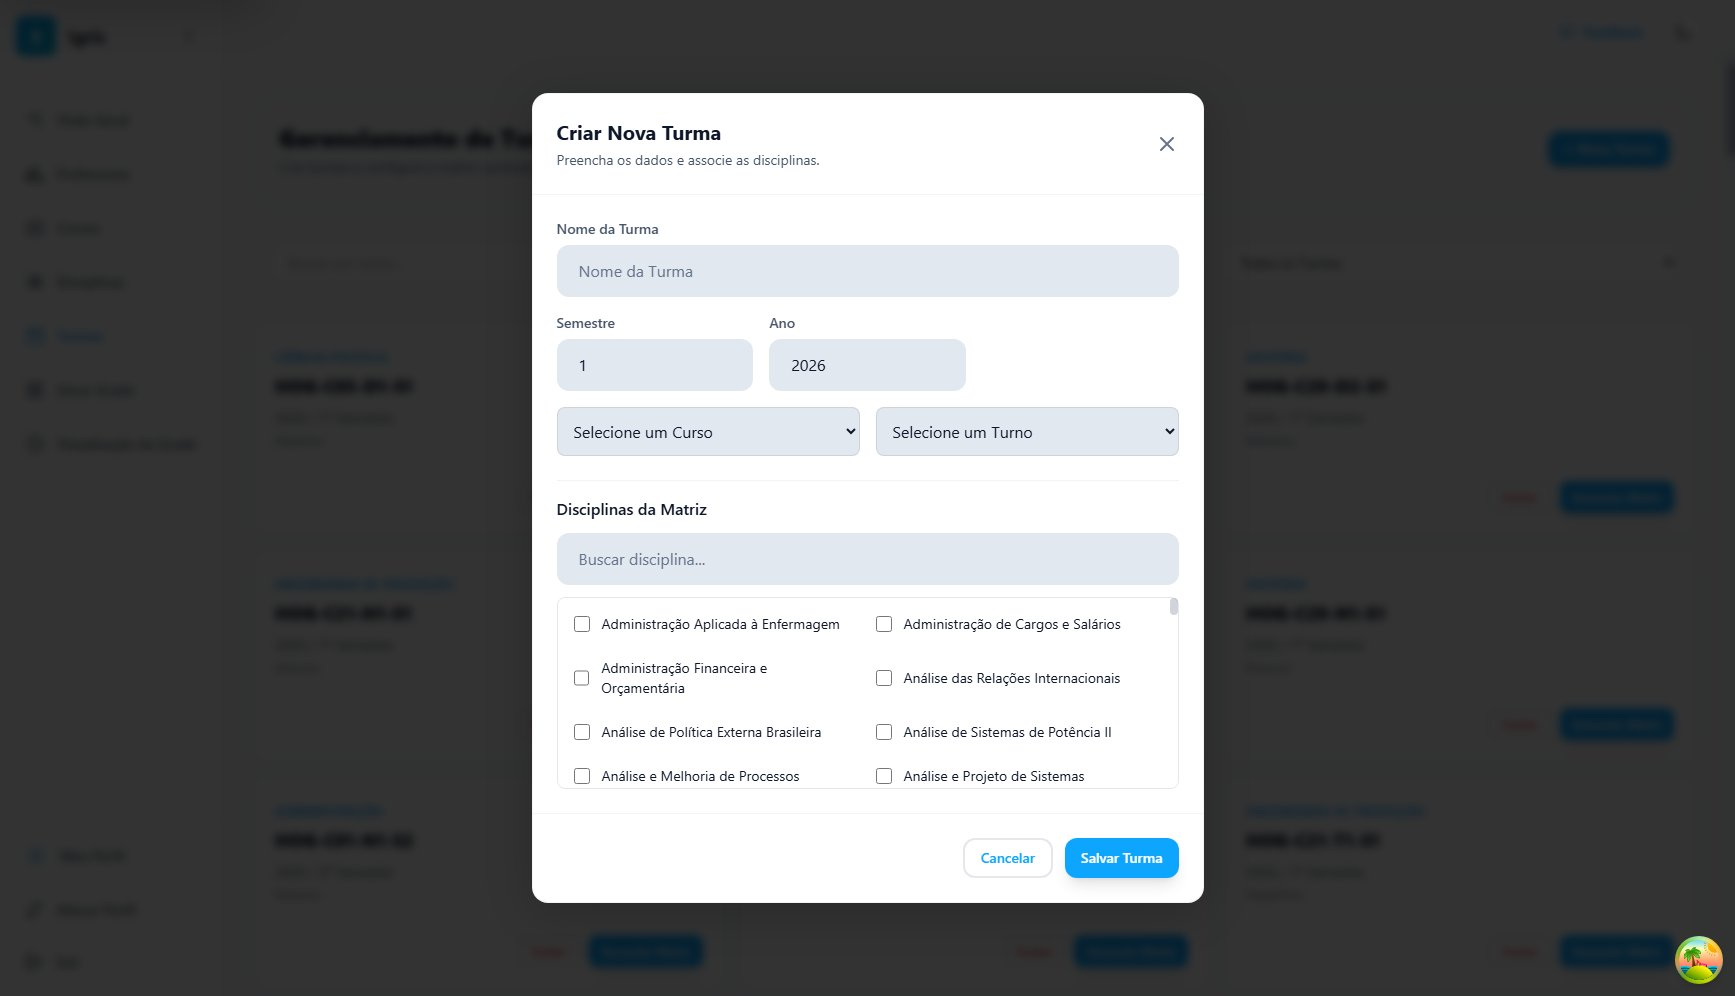
\includegraphics[width=\textwidth]{figuras/paginas/Figura_29_PG13.jpg}
\fonteautores
\end{figure}

A tela "Criar Nova Turma" funciona como um formulário em formato modal onde o usuário insere o nome, período, curso e turno da turma a ser criada. Simultaneamente, o usuário pode associar as disciplinas da matriz utilizando uma lista com caixas de seleção.

\begin{tabelainteracoes}{Interações da Criação de Nova Turma}{tab:interacoes-criacao-turma}
Informar o nome da turma & O sistema registra o nome ou código que identificará o novo grupo acadêmico. & O campo é obrigatório e deve evitar duplicidade dentro do mesmo período e contexto institucional. \\
\hline
Informar semestre e ano & O sistema define o período letivo ao qual a turma pertencerá. & Os valores devem representar um período válido; o ano deve ser numérico e o semestre deve estar entre as opções permitidas. \\
\hline
Selecionar curso e turno & O sistema vincula a turma ao curso e ao turno escolhidos. & Ambos os campos são obrigatórios e devem conter somente opções autorizadas para a coordenação ativa. \\
\hline
Pesquisar, marcar ou desmarcar disciplinas & O sistema monta temporariamente a matriz inicial da nova turma. & As seleções devem pertencer ao curso escolhido e somente serão persistidas com a criação da turma. \\
\hline
Clicar em ``Salvar Turma'' & O sistema valida os dados, cria a turma e salva os vínculos da matriz. & Em caso de sucesso, a janela é fechada e a listagem atualizada; dados inválidos devem ser destacados sem criar registros parciais. \\
\hline
Clicar em ``Cancelar'' ou fechar a janela & O sistema abandona o preenchimento e retorna ao gerenciamento de turmas. & Nenhuma turma ou matriz deve ser criada. \\
\hline
\end{tabelainteracoes}

% PG14.jpg
\begin{figure}[H]
\centering
\caption{Motor de Alocação - Configuração Inicial}
\label{fig:PG14}
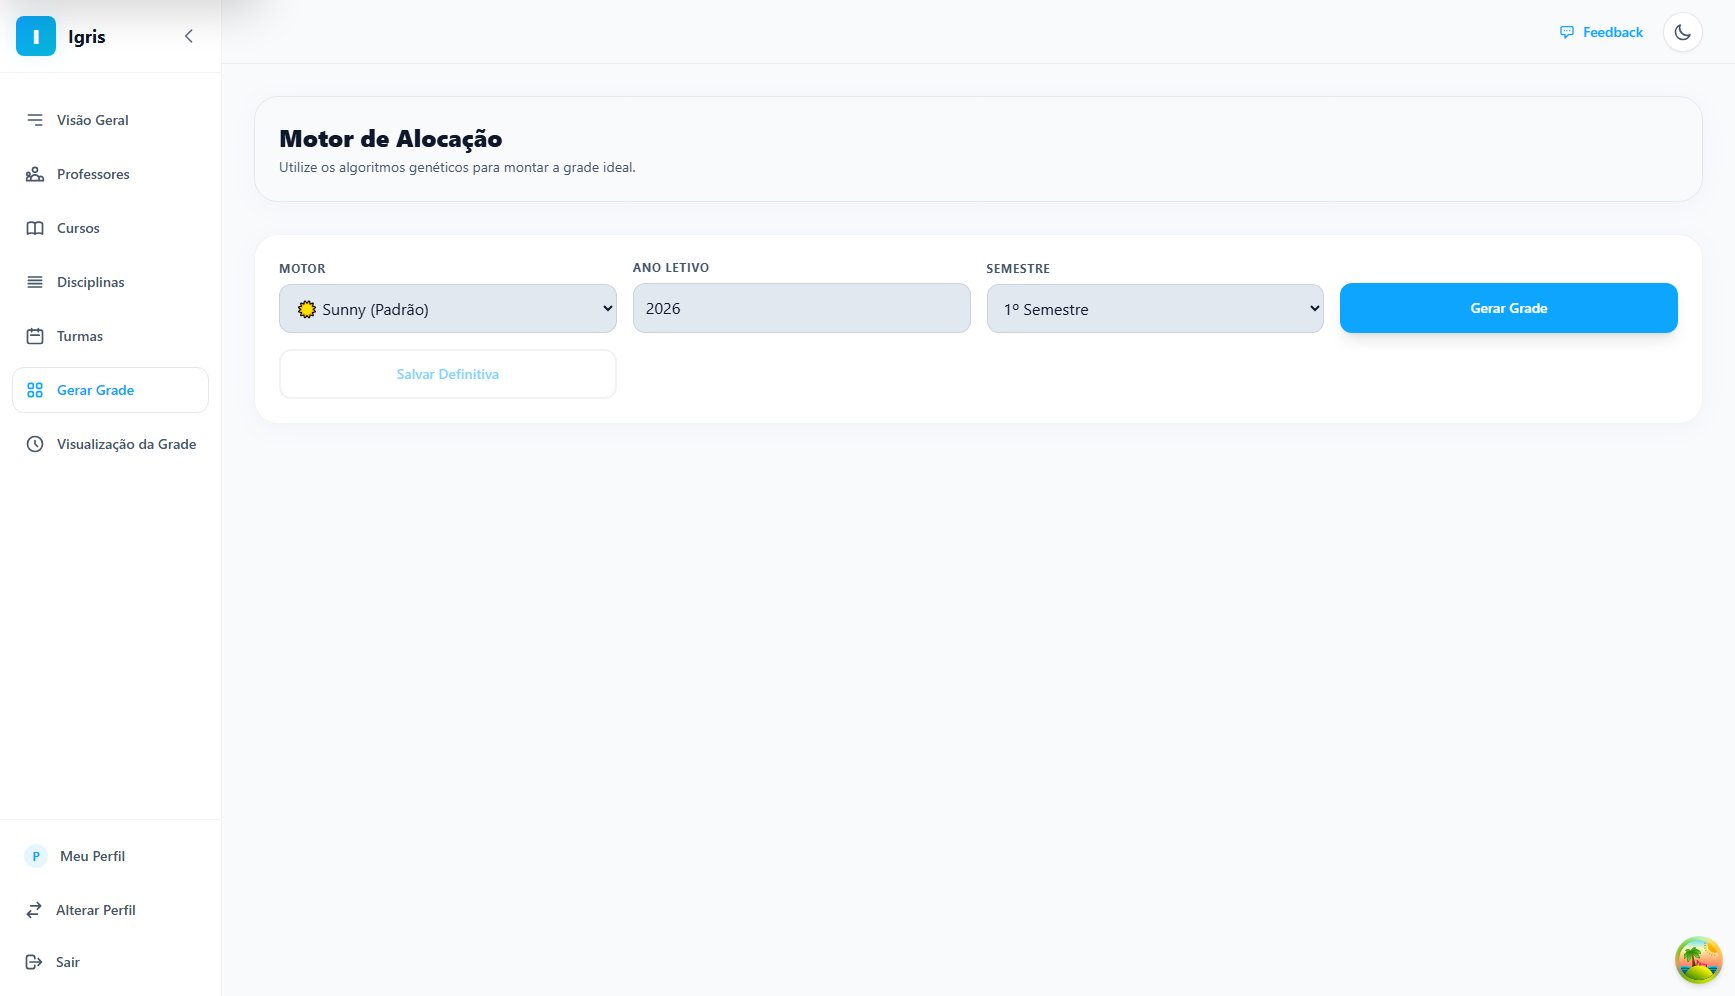
\includegraphics[width=\textwidth]{figuras/paginas/Figura_30_PG14.jpg}
\fonteautores
\end{figure}

A tela do Motor de Alocação é onde a geração da grade horária ocorre. O usuário seleciona o modelo de algoritmo desejado, como o Sunny (Padrão), além de especificar o ano letivo e o semestre, iniciando então o processamento com o botão "Gerar Grade".

\begin{tabelainteracoes}{Interações do Motor de Alocação -- Configuração Inicial}{tab:interacoes-motor-configuracao}
Selecionar o modelo de algoritmo & O sistema define o motor que processará a geração da grade. & Somente modelos disponíveis e configurados, como Sunny ou Morpheus, devem ser apresentados. \\
\hline
Informar o ano letivo & O sistema utiliza o ano para identificar turmas, matrizes e disponibilidades aplicáveis. & O campo é obrigatório e deve aceitar apenas um ano válido. \\
\hline
Selecionar o semestre & O sistema restringe a geração ao período letivo escolhido. & Deve ser selecionada uma das opções de semestre cadastradas. \\
\hline
Clicar em ``Gerar Grade'' & O sistema valida os dados, envia o problema ao motor selecionado e apresenta o estado de processamento. & O botão deve evitar solicitações duplicadas enquanto a execução estiver em andamento. \\
\hline
Tentar gerar sem dados acadêmicos suficientes & O sistema interrompe a operação e informa quais cadastros ou disponibilidades precisam ser completados. & Turmas sem matriz, disciplinas sem professor apto ou ausência de disponibilidade podem impedir ou comprometer a geração. \\
\hline
\end{tabelainteracoes}

% PG15.jpg
\begin{figure}[H]
\centering
\caption{Resultados do Motor de Alocação}
\label{fig:PG15}
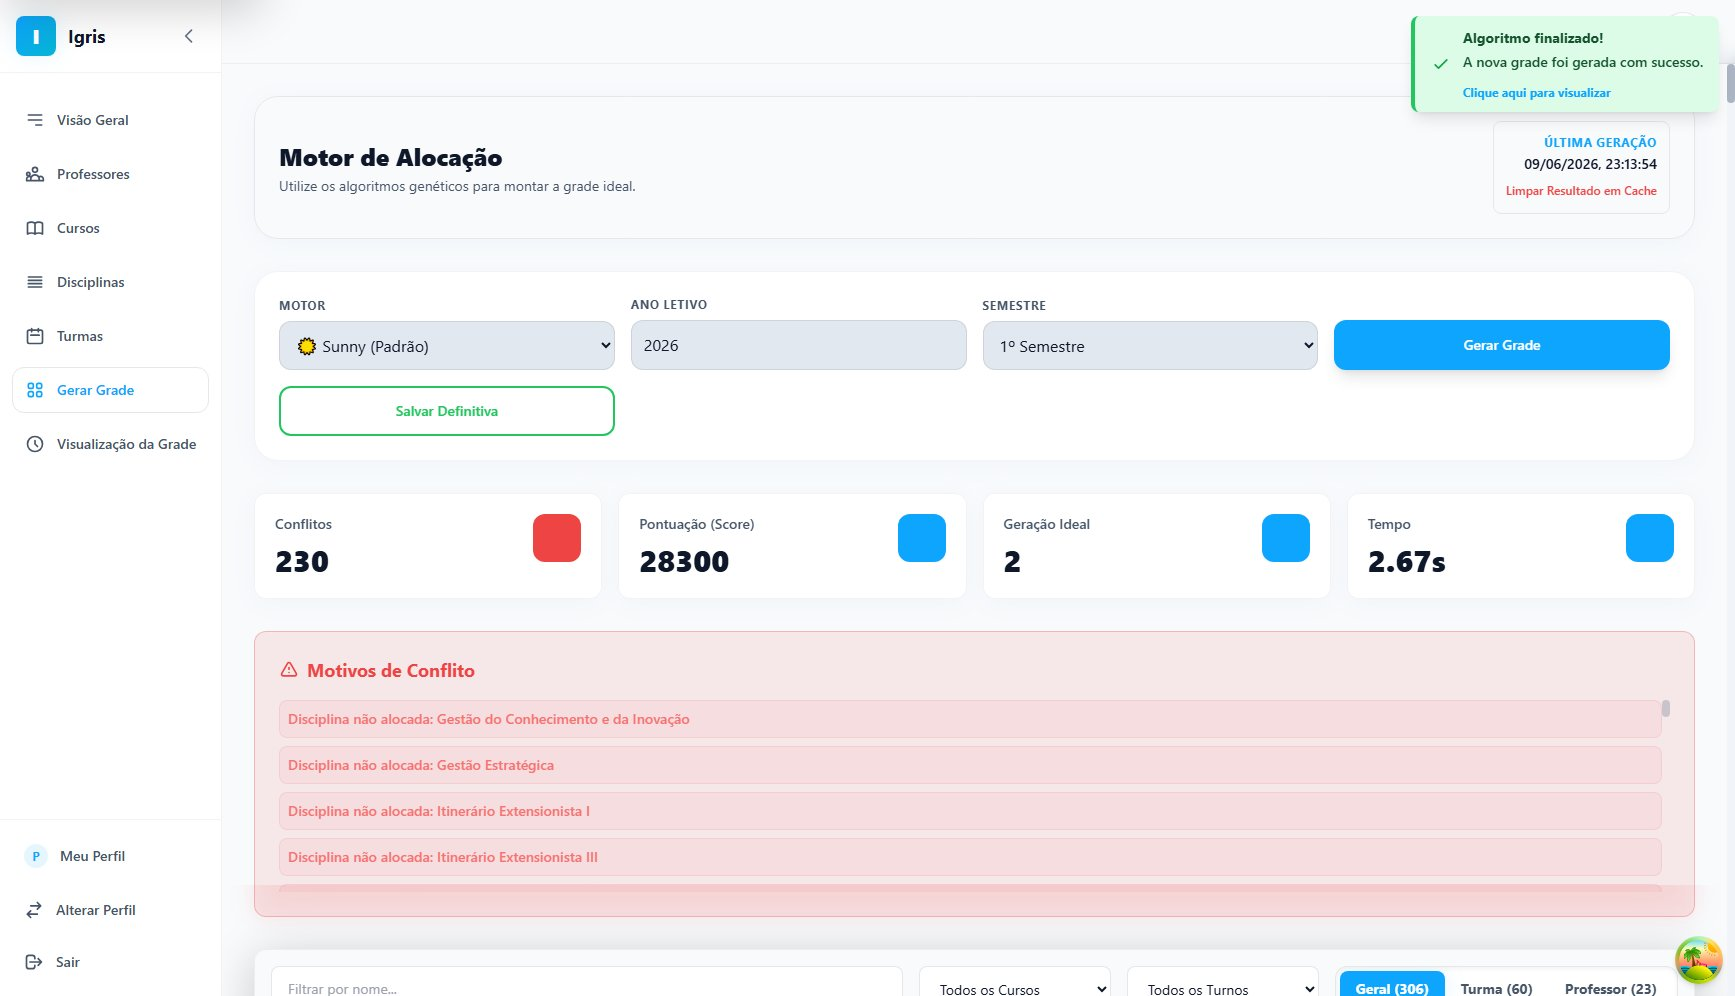
\includegraphics[width=\textwidth]{figuras/paginas/Figura_31_PG15.jpg}
\fonteautores
\end{figure}

Após o término da execução, o Motor de Alocação apresenta métricas valiosas como o número de conflitos restantes, a pontuação (score) obtida, a geração ideal e o tempo de execução do algoritmo. Uma área de alerta destaca as disciplinas que não puderam ser alocadas, indicando os gargalos.

\begin{tabelainteracoes}{Interações dos Resultados do Motor de Alocação}{tab:interacoes-resultados-motor}
Aguardar a conclusão do algoritmo & O sistema atualiza a tela com o resultado, as métricas de execução e uma notificação de término. & A interface deve distinguir claramente processamento, sucesso e falha. \\
\hline
Consultar conflitos, pontuação, geração e tempo & O sistema apresenta os indicadores produzidos pelo motor de alocação. & Os valores permitem avaliar a qualidade da solução e comparar diferentes configurações. \\
\hline
Consultar ``Motivos de Conflito'' & O sistema lista disciplinas e restrições que impediram determinadas alocações. & Os itens devem fornecer informação suficiente para que o gestor corrija cadastros, matrizes ou disponibilidades. \\
\hline
Clicar em ``Salvar Definitivo'' & O sistema solicita confirmação e persiste a grade e suas alocações. & Uma solução com conflitos deve exigir ciência do usuário ou ser bloqueada conforme a regra institucional. \\
\hline
Clicar em ``Gerar Novamente'' & O sistema inicia uma nova execução utilizando os parâmetros selecionados. & O resultado anterior não deve substituir uma grade já salva sem confirmação. \\
\hline
Ocorrer falha durante o processamento & O sistema informa que a geração não foi concluída e mantém os parâmetros para uma nova tentativa. & Nenhuma grade incompleta deve ser registrada como definitiva. \\
\hline
\end{tabelainteracoes}

% PG16.jpg
\begin{figure}[H]
\centering
\caption{Visualização Geral da Grade com Alertas}
\label{fig:PG16}
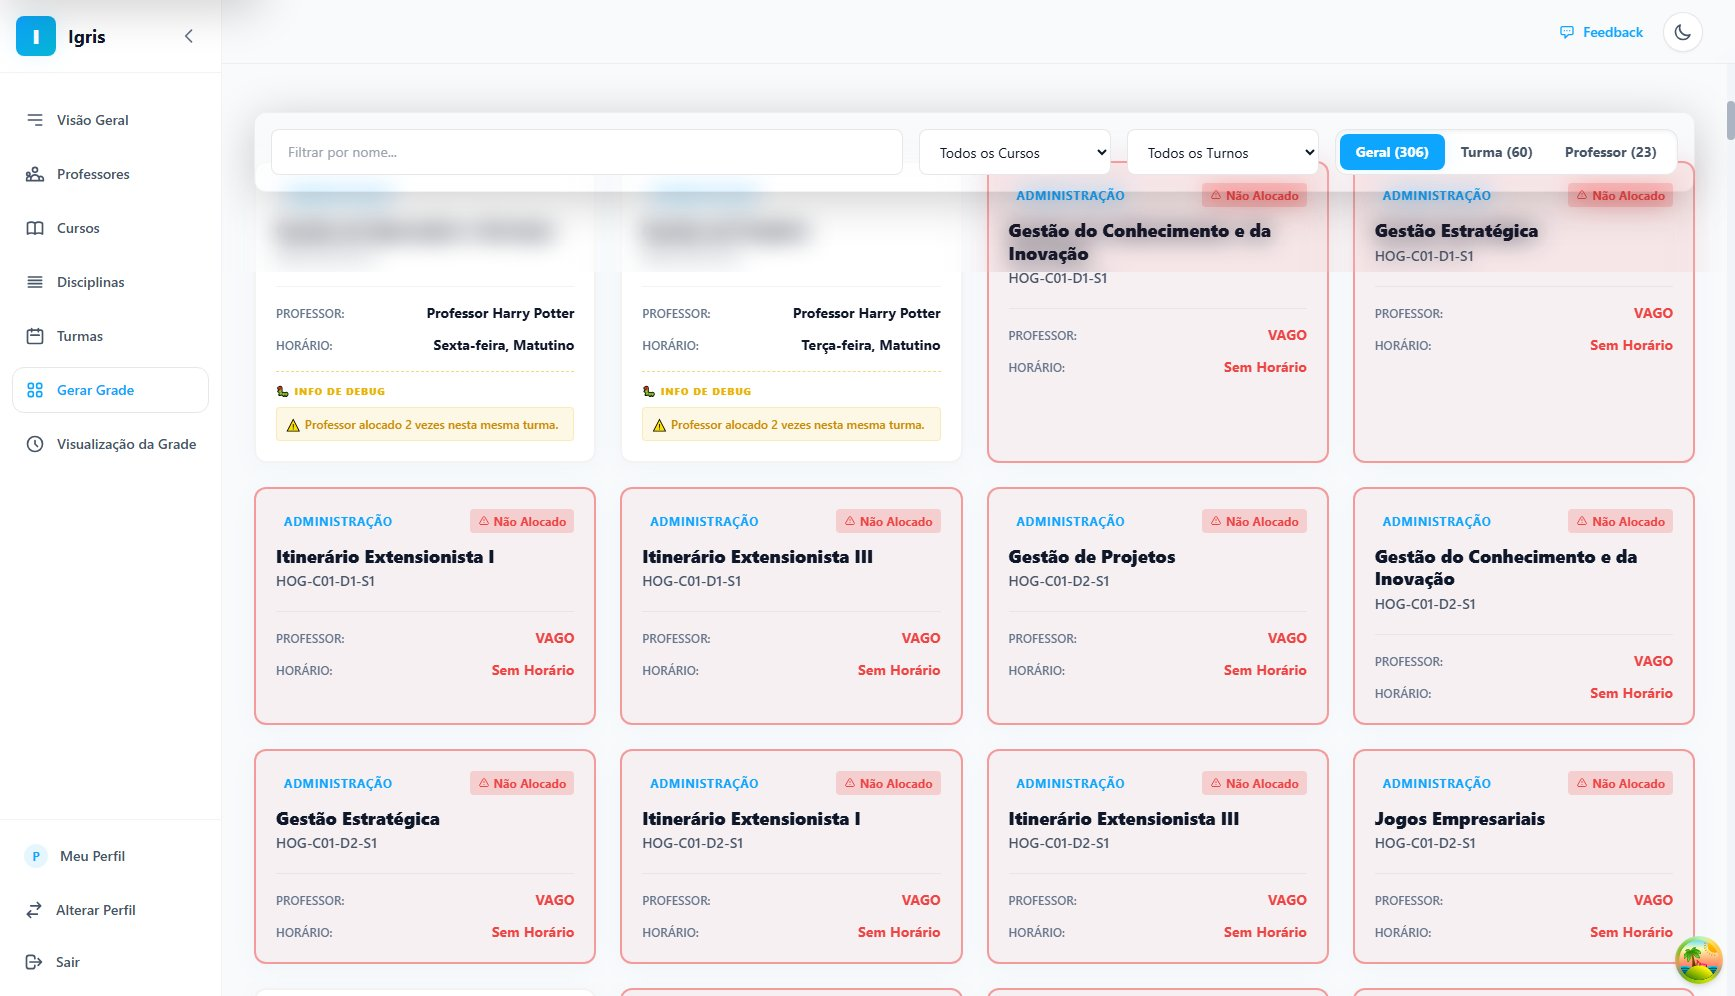
\includegraphics[width=\textwidth]{figuras/paginas/Figura_32_PG16.jpg}
\fonteautores
\end{figure}

A interface de Visualização da Grade possibilita a inspeção das aulas alocadas de forma generalizada. Ela apresenta as interações entre disciplinas, turmas e professores, destacando claramente em vermelho situações onde uma disciplina permanece "Não Alocada" ou quando faltam horários.

\begin{tabelainteracoes}{Interações da Visualização Geral da Grade com Alertas}{tab:interacoes-grade-alertas}
Pesquisar uma turma, disciplina ou professor & O sistema filtra os cartões da grade conforme o termo informado. & A busca deve abranger os dados relevantes exibidos em cada alocação. \\
\hline
Selecionar curso ou turno & O sistema exibe somente as alocações compatíveis com os filtros escolhidos. & Os filtros podem ser combinados e não alteram a grade armazenada. \\
\hline
Alternar entre as visões Geral, Turmas e Professores & O sistema reorganiza os mesmos dados conforme a perspectiva escolhida. & A quantidade indicada em cada aba deve refletir os registros disponíveis. \\
\hline
Visualizar um cartão destacado em vermelho & O sistema apresenta a disciplina como não alocada ou sem horário definido. & O alerta indica pendência que deve ser tratada antes da validação definitiva da grade. \\
\hline
Consultar o motivo de uma pendência & O sistema apresenta as informações disponíveis sobre professor, turma, horário ou restrição conflitante. & A ausência de professor apto ou de disponibilidade deve ser explicitada quando identificável. \\
\hline
\end{tabelainteracoes}

% PG17.jpg
\begin{figure}[H]
\centering
\caption{Grade Horária - Visão por Turma (Cartões)}
\label{fig:PG17}
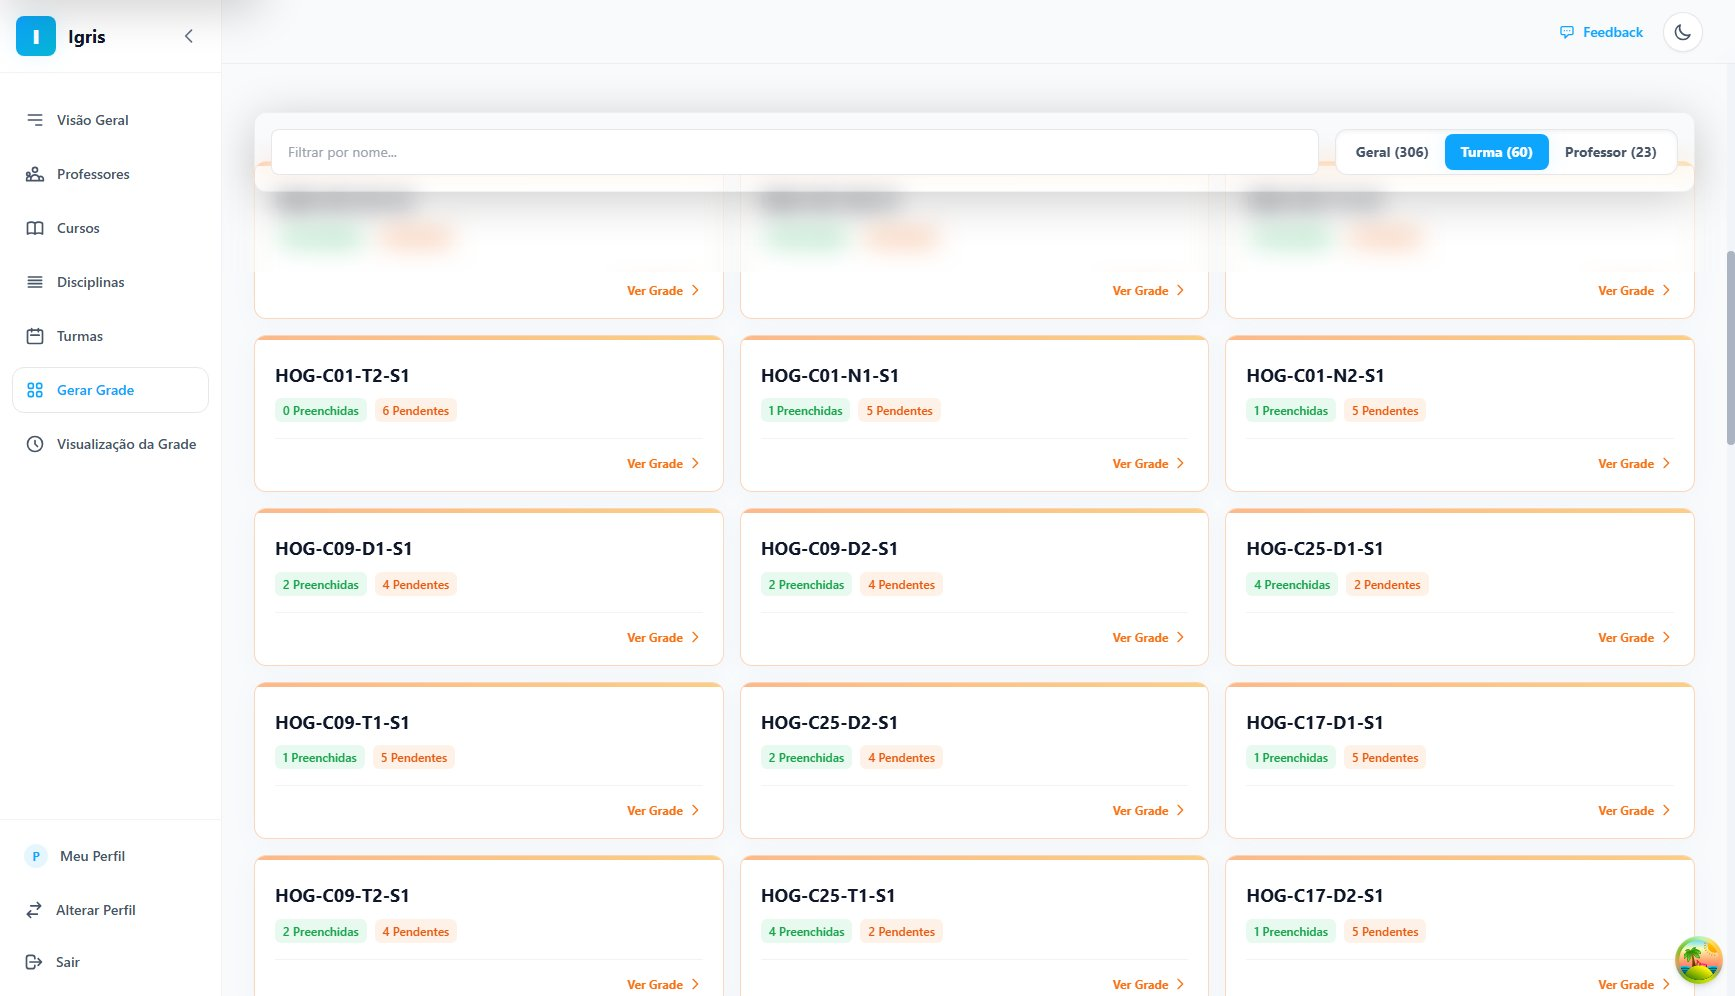
\includegraphics[width=\textwidth]{figuras/paginas/Figura_33_PG17.jpg}
\fonteautores
\end{figure}

A Grade Horária pode ser vista sob a perspectiva das turmas. Em formato de cartões, o coordenador pode avaliar o status de cada turma (ex: 3 Preenchidas, 1 Pendentes), facilitando a identificação das classes que precisam de intervenções.

\begin{tabelainteracoes}{Interações da Grade Horária -- Visão por Turma}{tab:interacoes-grade-por-turma}
Selecionar a aba ``Turmas'' & O sistema agrupa as alocações em cartões correspondentes a cada turma. & Cada cartão deve resumir a quantidade de horários preenchidos e pendentes. \\
\hline
Pesquisar uma turma & O sistema filtra os cartões pelo nome ou identificador informado. & A pesquisa não modifica as alocações existentes. \\
\hline
Clicar em ``Ver Grade'' & O sistema abre a matriz semanal detalhada da turma selecionada. & O detalhamento deve apresentar somente aulas e pendências relacionadas à turma acionada. \\
\hline
Visualizar o indicador de pendências & O sistema destaca a quantidade de componentes ainda não alocados. & A cor e o texto do indicador devem permitir diferenciar uma grade completa de uma incompleta. \\
\hline
Não existir grade para o período & O sistema informa que não há dados disponíveis para exibição. & O usuário pode ser orientado a gerar ou selecionar outra grade. \\
\hline
\end{tabelainteracoes}

% PG18.jpg
\begin{figure}[H]
\centering
\caption{Detalhamento da Matriz Semanal de uma Turma}
\label{fig:PG18}
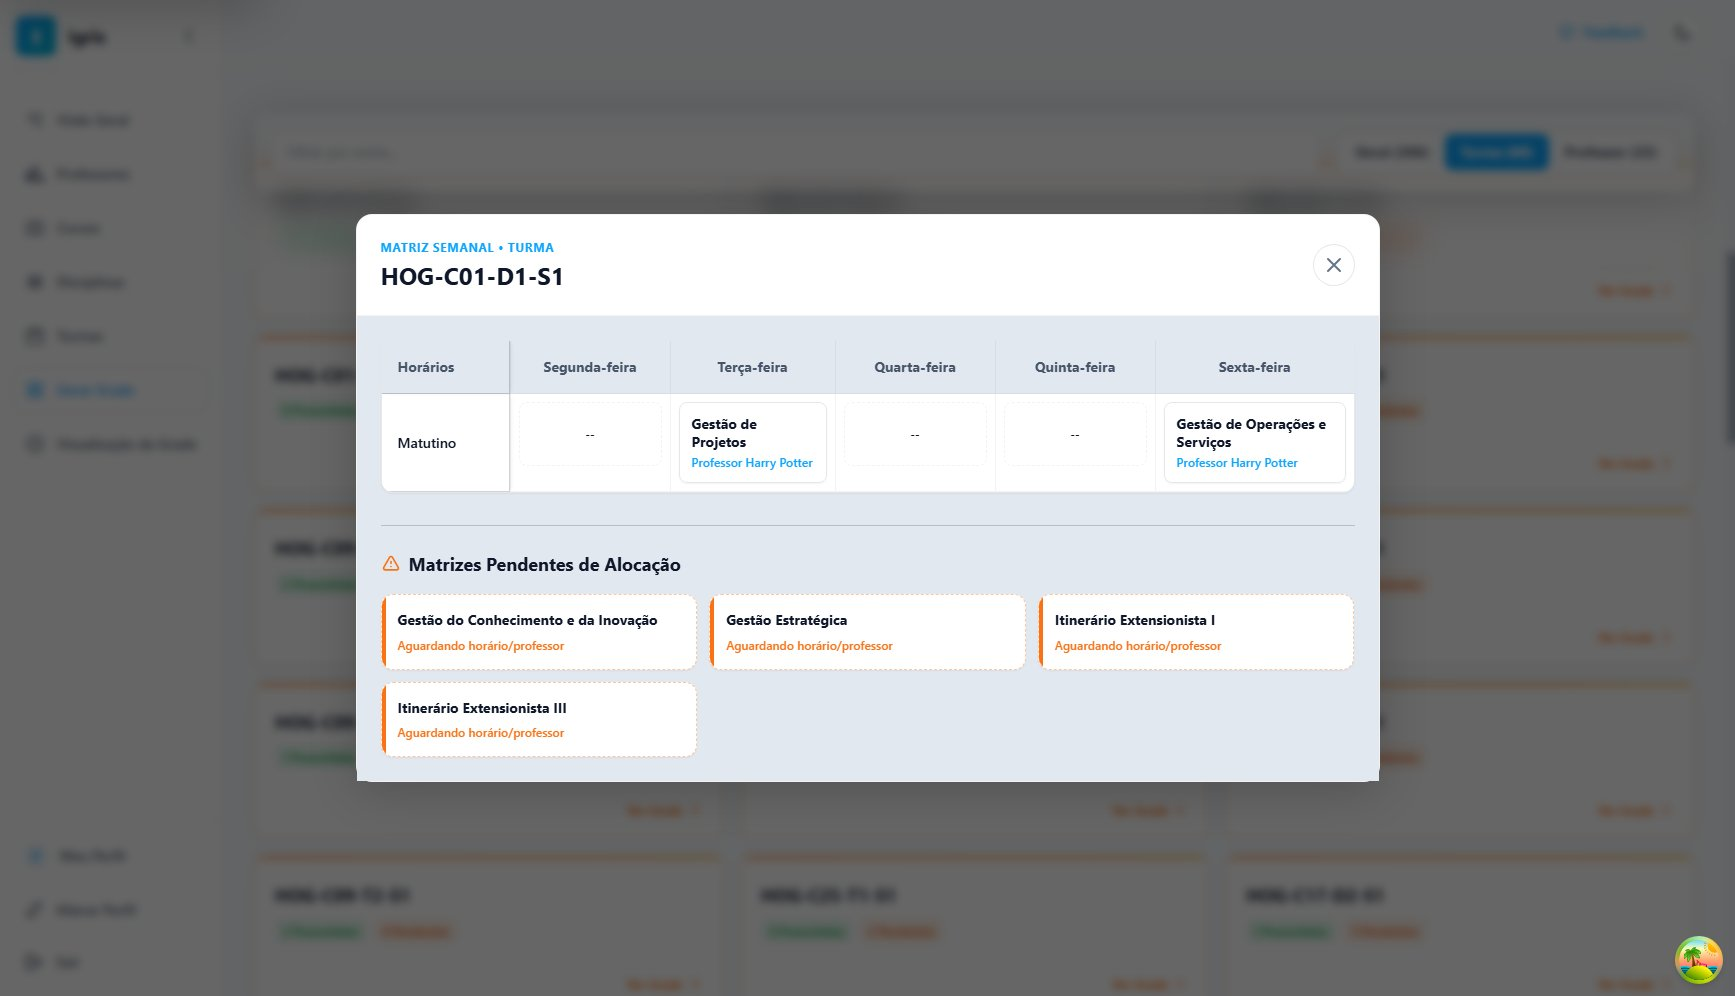
\includegraphics[width=\textwidth]{figuras/paginas/Figura_34_PG18.jpg}
\fonteautores
\end{figure}

Ao clicar em uma turma, um detalhamento semanal é exibido. A janela cruza os dias da semana e turnos mostrando as disciplinas e seus respectivos professores alocados para aquela turma, facilitando a visualização.

\begin{tabelainteracoes}{Interações do Detalhamento Semanal de uma Turma}{tab:interacoes-detalhamento-turma}
Abrir o detalhamento de uma turma & O sistema apresenta uma matriz com dias da semana, turnos, disciplinas e professores alocados. & O cabeçalho deve identificar claramente a turma consultada. \\
\hline
Consultar uma célula preenchida & O sistema exibe a disciplina e o professor designados para aquele dia e turno. & Uma mesma turma não pode possuir duas aulas simultâneas no mesmo intervalo. \\
\hline
Consultar uma célula vazia & O sistema indica que não há aula alocada naquele período. & A célula vazia pode representar horário livre, conforme a matriz e a carga horária previstas. \\
\hline
Consultar ``Matrizes Pendentes de Alocação'' & O sistema lista as disciplinas da turma que ainda não receberam horário ou professor. & As pendências devem permanecer visíveis até que uma nova geração ou correção seja realizada. \\
\hline
Clicar no ícone de fechar & O sistema encerra o detalhamento e retorna à visão por turmas. & Os dados são apenas consultados; fechar a janela não altera a grade. \\
\hline
\end{tabelainteracoes}

% PG19.jpg
\begin{figure}[H]
\centering
\caption{Grade Horária - Visão por Professor}
\label{fig:PG19}
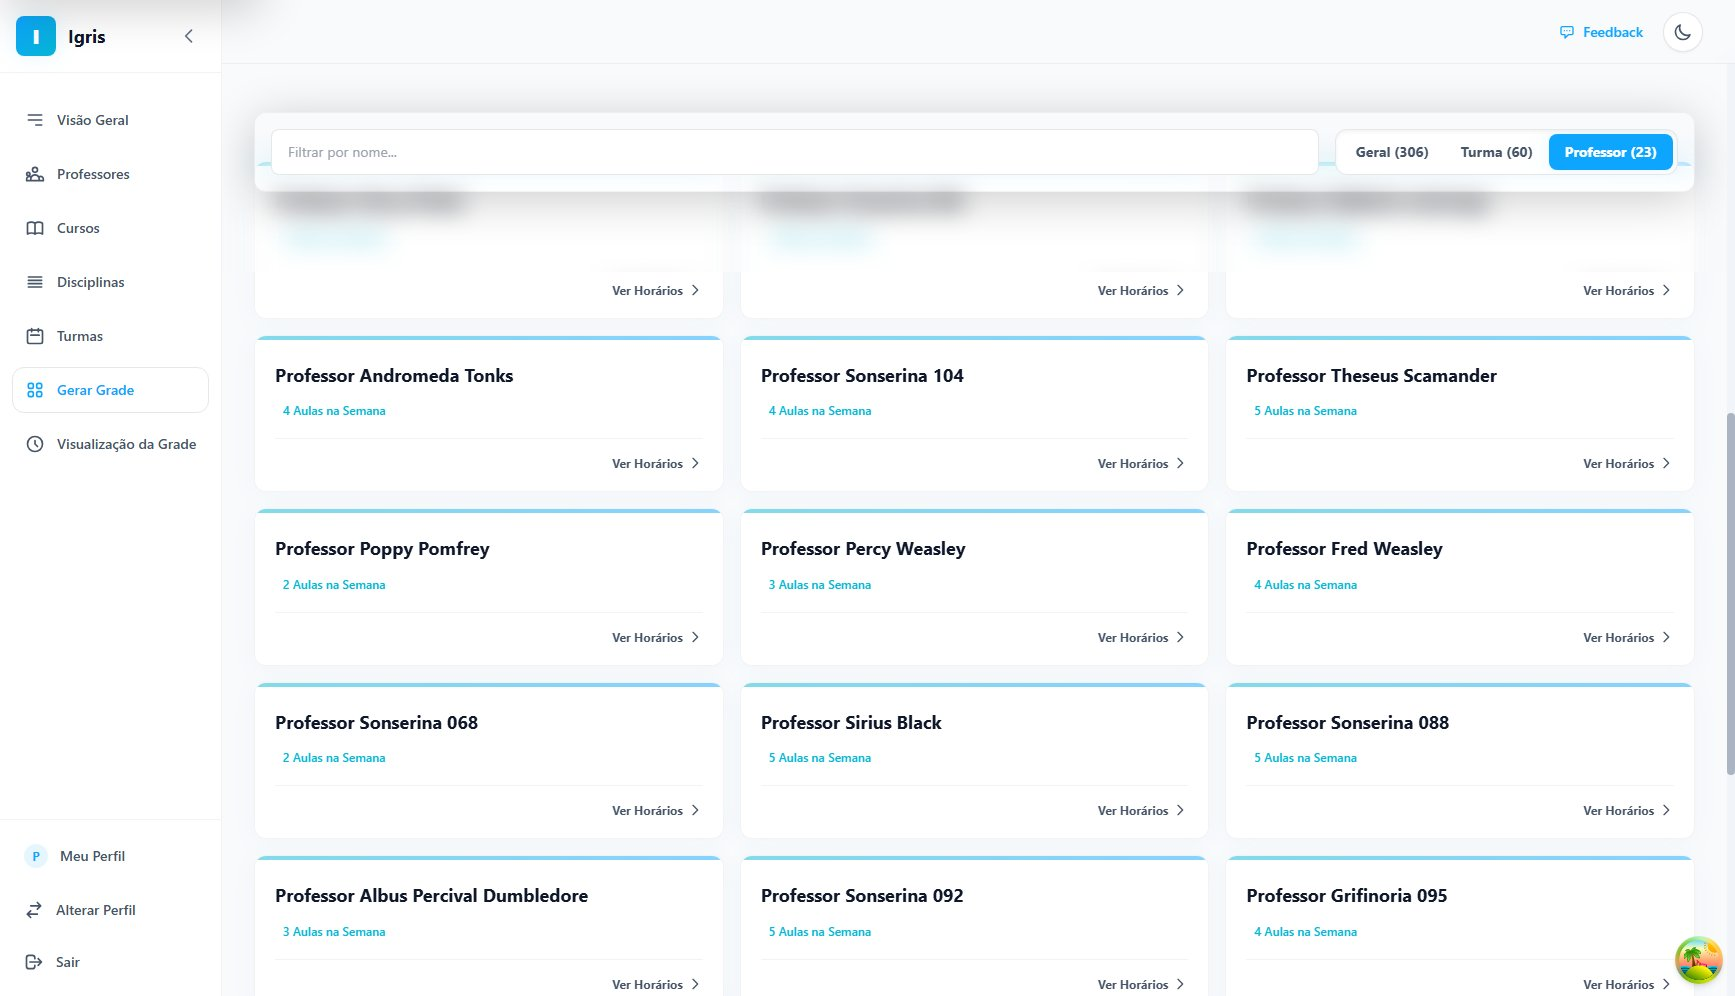
\includegraphics[width=\textwidth]{figuras/paginas/Figura_35_PG19.jpg}
\fonteautores
\end{figure}

A visão por professor exibe o total de aulas designadas na semana para cada docente. Os cartões fornecem um panorama rápido da carga horária que foi alocada a eles, essencial para a validação da adequação aos contratos de trabalho.

\begin{tabelainteracoes}{Interações da Grade Horária -- Visão por Professor}{tab:interacoes-grade-por-professor}
Selecionar a aba ``Professores'' & O sistema agrupa as aulas por docente e apresenta um cartão para cada professor. & A contagem exibida deve considerar somente a grade e o período selecionados. \\
\hline
Pesquisar um professor & O sistema filtra os cartões conforme o nome informado. & Quando não houver resultado, deve ser exibido um estado de lista vazia. \\
\hline
Consultar a quantidade de aulas da semana & O sistema mostra a carga semanal atribuída ao professor. & O indicador auxilia a identificar subalocação ou excesso de carga, mas deve ser comparado às regras contratuais cadastradas. \\
\hline
Clicar em ``Ver Horários'' & O sistema abre a matriz semanal individual do professor selecionado. & A janela deve apresentar apenas as alocações vinculadas ao docente acionado. \\
\hline
Identificar sobreposição de aulas & O sistema destaca ou informa o conflito de horários do professor. & Um docente não pode ser alocado simultaneamente em turmas diferentes. \\
\hline
\end{tabelainteracoes}

% PG20.jpg
\begin{figure}[H]
\centering
\caption{Detalhamento da Matriz Semanal de um Professor}
\label{fig:PG20}
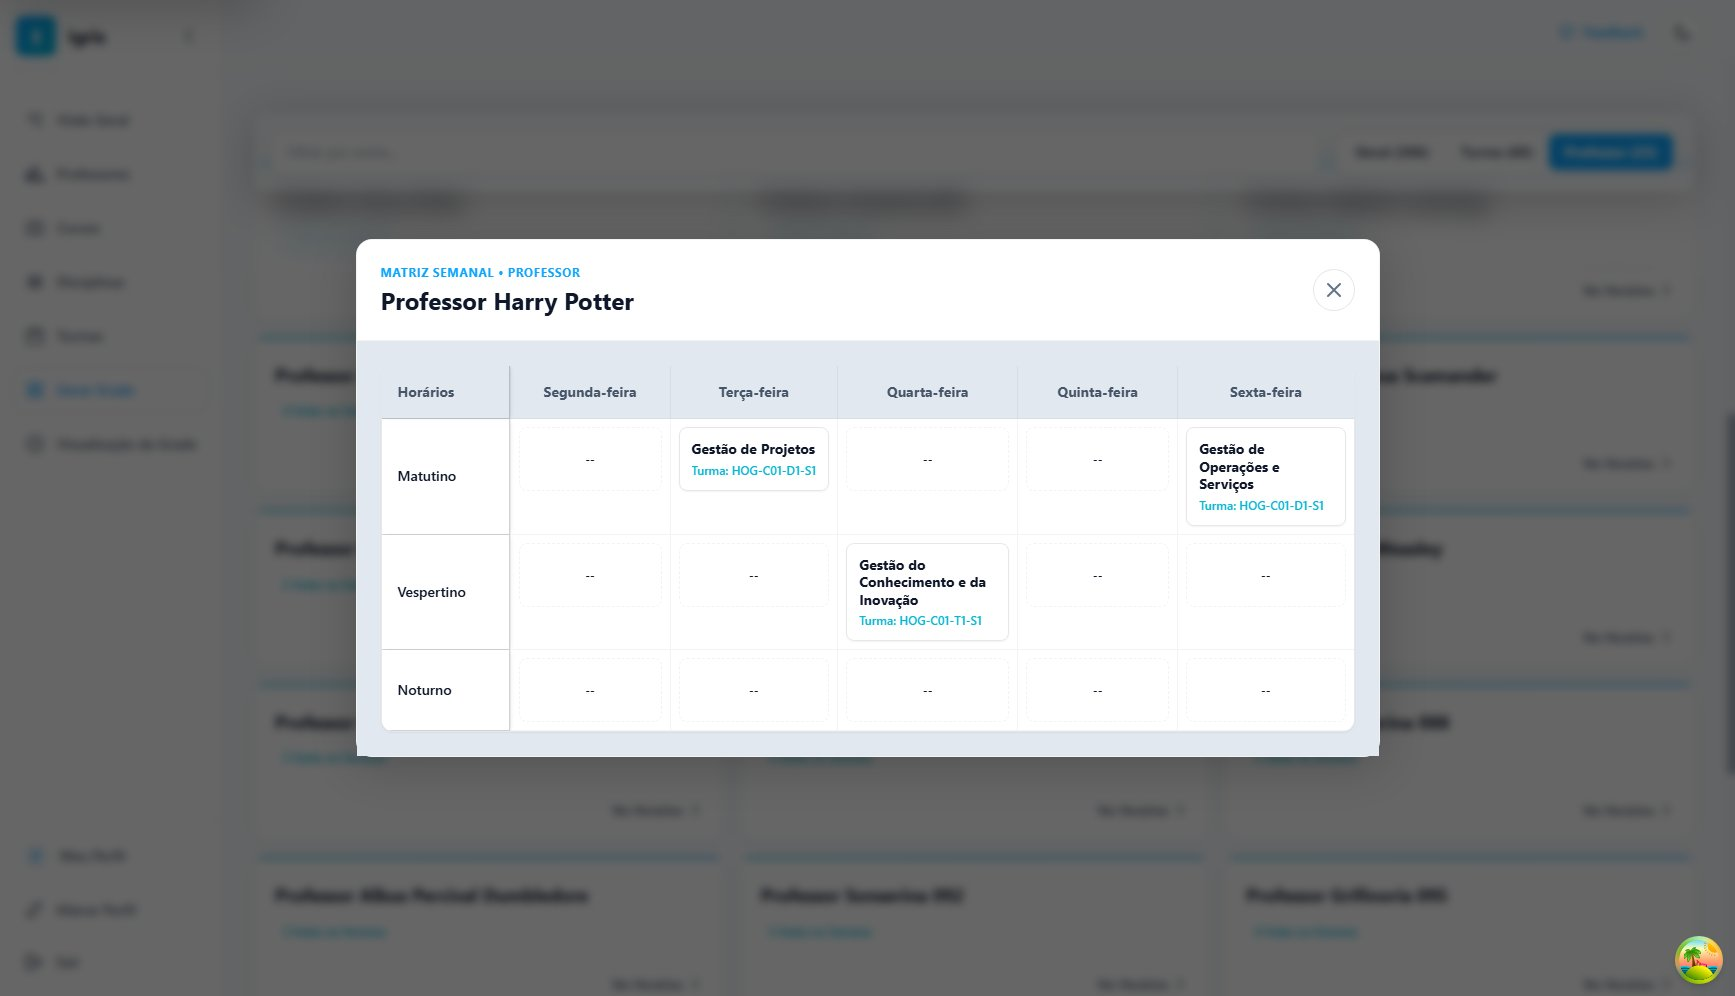
\includegraphics[width=\textwidth]{figuras/paginas/Figura_36_PG20.jpg}
\fonteautores
\end{figure}

Clicar sobre o cartão de um professor exibe a sua matriz semanal. O sistema apresenta em quais dias e horários o professor estará lecionando, junto com as disciplinas e turmas para as quais ele foi designado.

\begin{tabelainteracoes}{Interações do Detalhamento Semanal de um Professor}{tab:interacoes-detalhamento-professor}
Abrir os horários de um professor & O sistema apresenta a matriz semanal individual, organizada por dias e turnos. & O cabeçalho deve indicar o nome do docente consultado. \\
\hline
Consultar uma aula alocada & O sistema exibe a disciplina e a turma correspondentes ao horário. & A alocação deve respeitar a disponibilidade e as áreas de atuação cadastradas para o professor. \\
\hline
Consultar um período sem aula & O sistema mantém a célula vazia ou a identifica como livre. & A ausência de aula não significa necessariamente disponibilidade, pois pode existir uma restrição cadastrada. \\
\hline
Detectar duas aulas no mesmo horário & O sistema deve sinalizar a inconsistência para correção. & Sobreposições representam conflito impeditivo na grade do docente. \\
\hline
Clicar no ícone de fechar & O sistema fecha a matriz individual e retorna à visão por professores. & A consulta não modifica as alocações. \\
\hline
\end{tabelainteracoes}

% PG21.jpg
\begin{figure}[H]
\centering
\caption{Acompanhamento Geral das Pendências}
\label{fig:PG21}
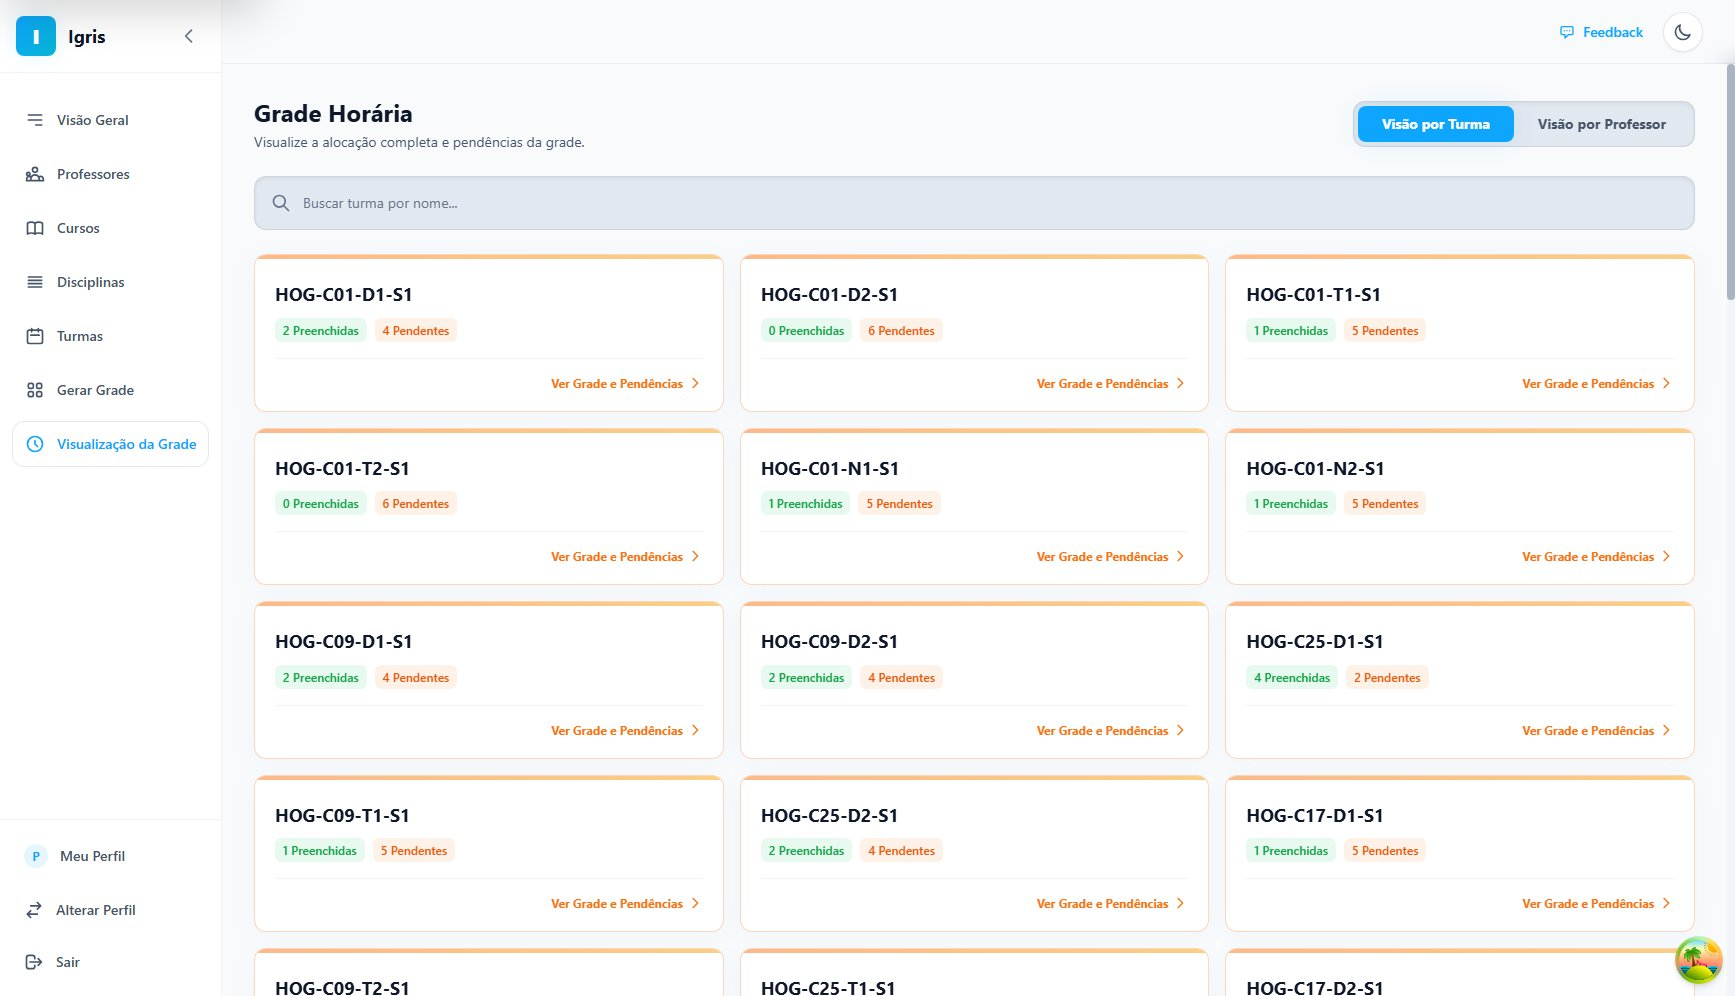
\includegraphics[width=\textwidth]{figuras/paginas/Figura_37_PG21.jpg}
\fonteautores
\end{figure}

A visão por turma na Grade Horária reforça a visualização em cartões, permitindo uma alternância ágil entre a visão de turmas e de professores, sempre indicando em destaque onde existem pendências e horários preenchidos.

\begin{tabelainteracoes}{Interações do Acompanhamento Geral das Pendências}{tab:interacoes-acompanhamento-pendencias}
Alternar entre ``Visão por Turma'' e ``Visão por Professor'' & O sistema reorganiza a grade pela perspectiva escolhida. & A alternância não executa nova geração nem modifica os dados salvos. \\
\hline
Pesquisar pelo nome & O sistema filtra a relação de turmas ou professores da visão ativa. & O campo deve ser limpo ou reaplicado corretamente ao trocar de visão. \\
\hline
Consultar indicadores de preenchimento e pendência & O sistema apresenta um resumo quantitativo em cada cartão. & Os valores devem ser atualizados sempre que uma nova grade for salva. \\
\hline
Clicar no detalhamento de um cartão & O sistema abre a matriz semanal e, quando aplicável, a lista de pendências. & O usuário deve conseguir identificar o item que exige intervenção. \\
\hline
Não haver pendências & O sistema apresenta os cartões como completos, sem alertas de alocação. & A ausência de pendências não dispensa a validação de carga e conflitos pelo gestor. \\
\hline
\end{tabelainteracoes}

% PG23.jpg
\begin{figure}[H]
\centering
\caption{Grade Horária - Detalhamento de Turma e Pendências}
\label{fig:PG23}
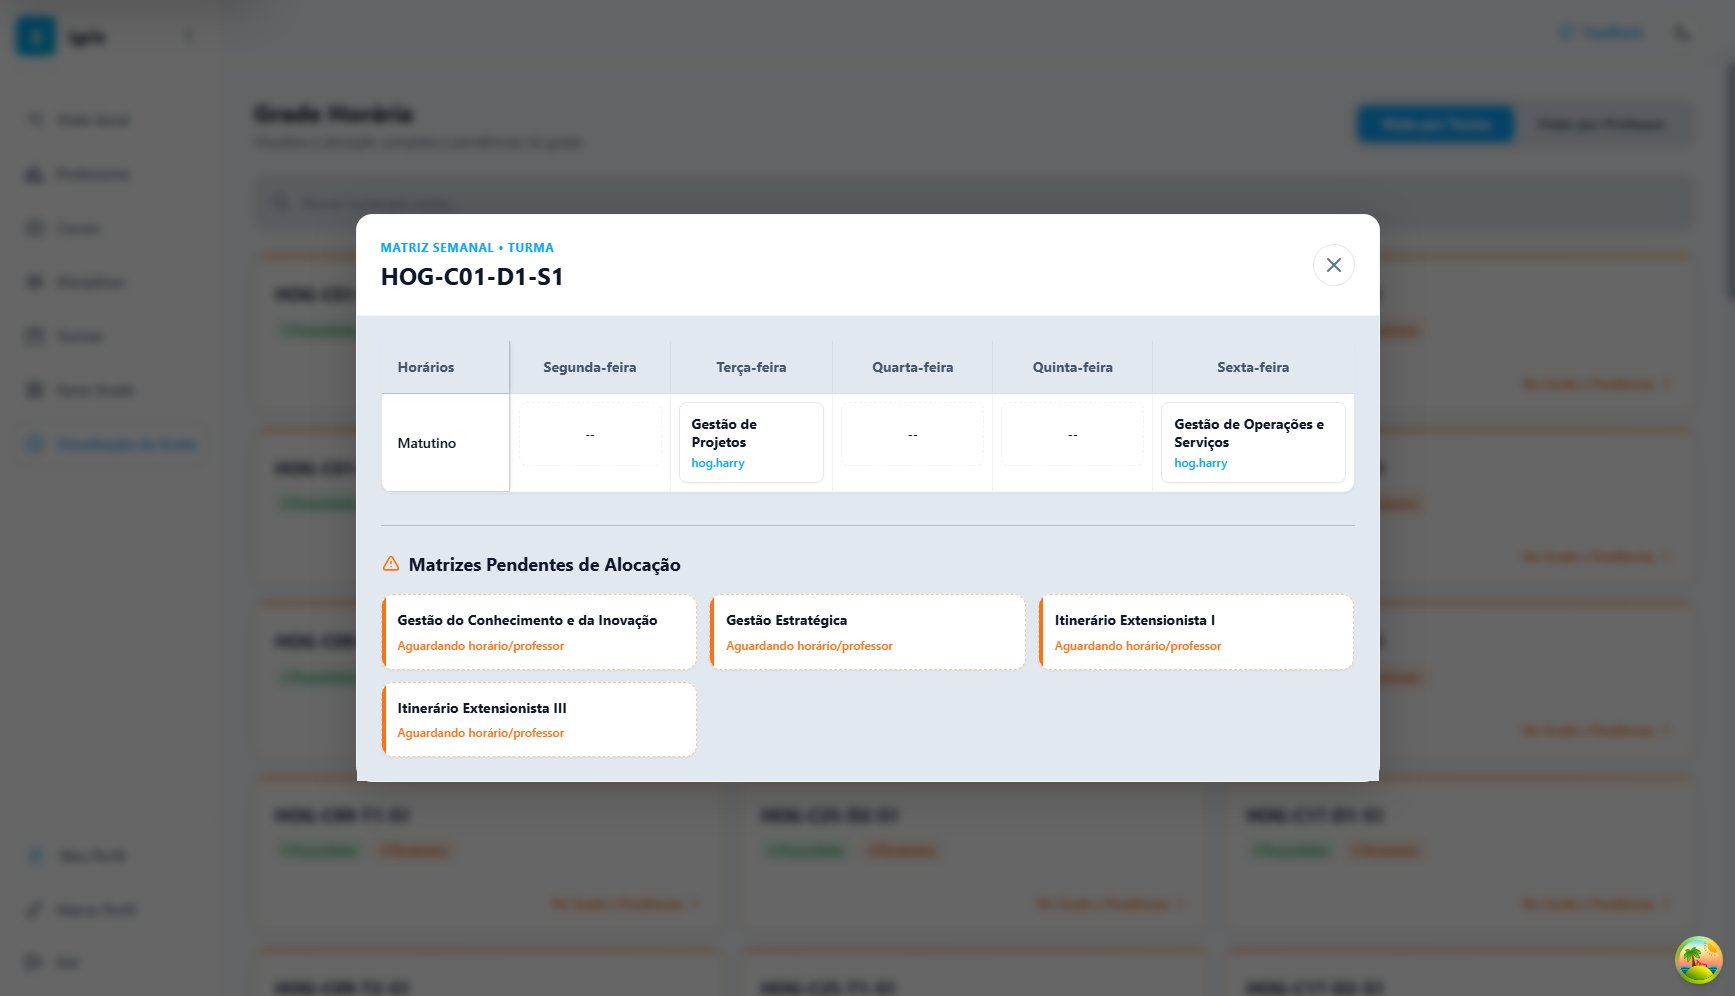
\includegraphics[width=\textwidth]{figuras/paginas/Figura_38_PG23.jpg}
\fonteautores
\end{figure}

A tela apresenta o detalhamento da grade semanal de uma turma selecionada. A matriz relaciona os dias da semana aos turnos e identifica as disciplinas, os professores e as turmas presentes em cada horário. Na parte inferior, a interface também reúne as disciplinas da matriz que ainda permanecem pendentes de alocação.

\begin{tabelainteracoes}{Interações do Detalhamento de Turma e Pendências}{tab:interacoes-detalhamento-turma-pendencias}
Abrir o detalhamento de uma turma & O sistema exibe a matriz semanal e identifica a turma selecionada no cabeçalho. & A consulta deve considerar a grade ativa e o período letivo correspondente. \\
\hline
Consultar uma célula preenchida & O sistema apresenta a disciplina e o professor alocados no respectivo dia e turno. & Uma turma não pode possuir duas disciplinas no mesmo intervalo de horário. \\
\hline
Consultar uma célula vazia & O sistema indica que não existe aula alocada naquele período. & O espaço vazio pode representar um horário livre ou uma carga horária ainda não distribuída. \\
\hline
Consultar ``Matrizes Pendentes de Alocação'' & O sistema lista as disciplinas da turma que ainda não receberam um horário válido. & As pendências auxiliam o coordenador a identificar restrições que exigem correção ou uma nova geração da grade. \\
\hline
Clicar no ícone de fechar & O sistema encerra a janela e retorna à visão geral das turmas. & A operação é apenas de consulta e não altera a grade. \\
\hline
\end{tabelainteracoes}

% PG24.jpg
\begin{figure}[H]
\centering
\caption{Grade Horária - Visão por Professor}
\label{fig:PG24}
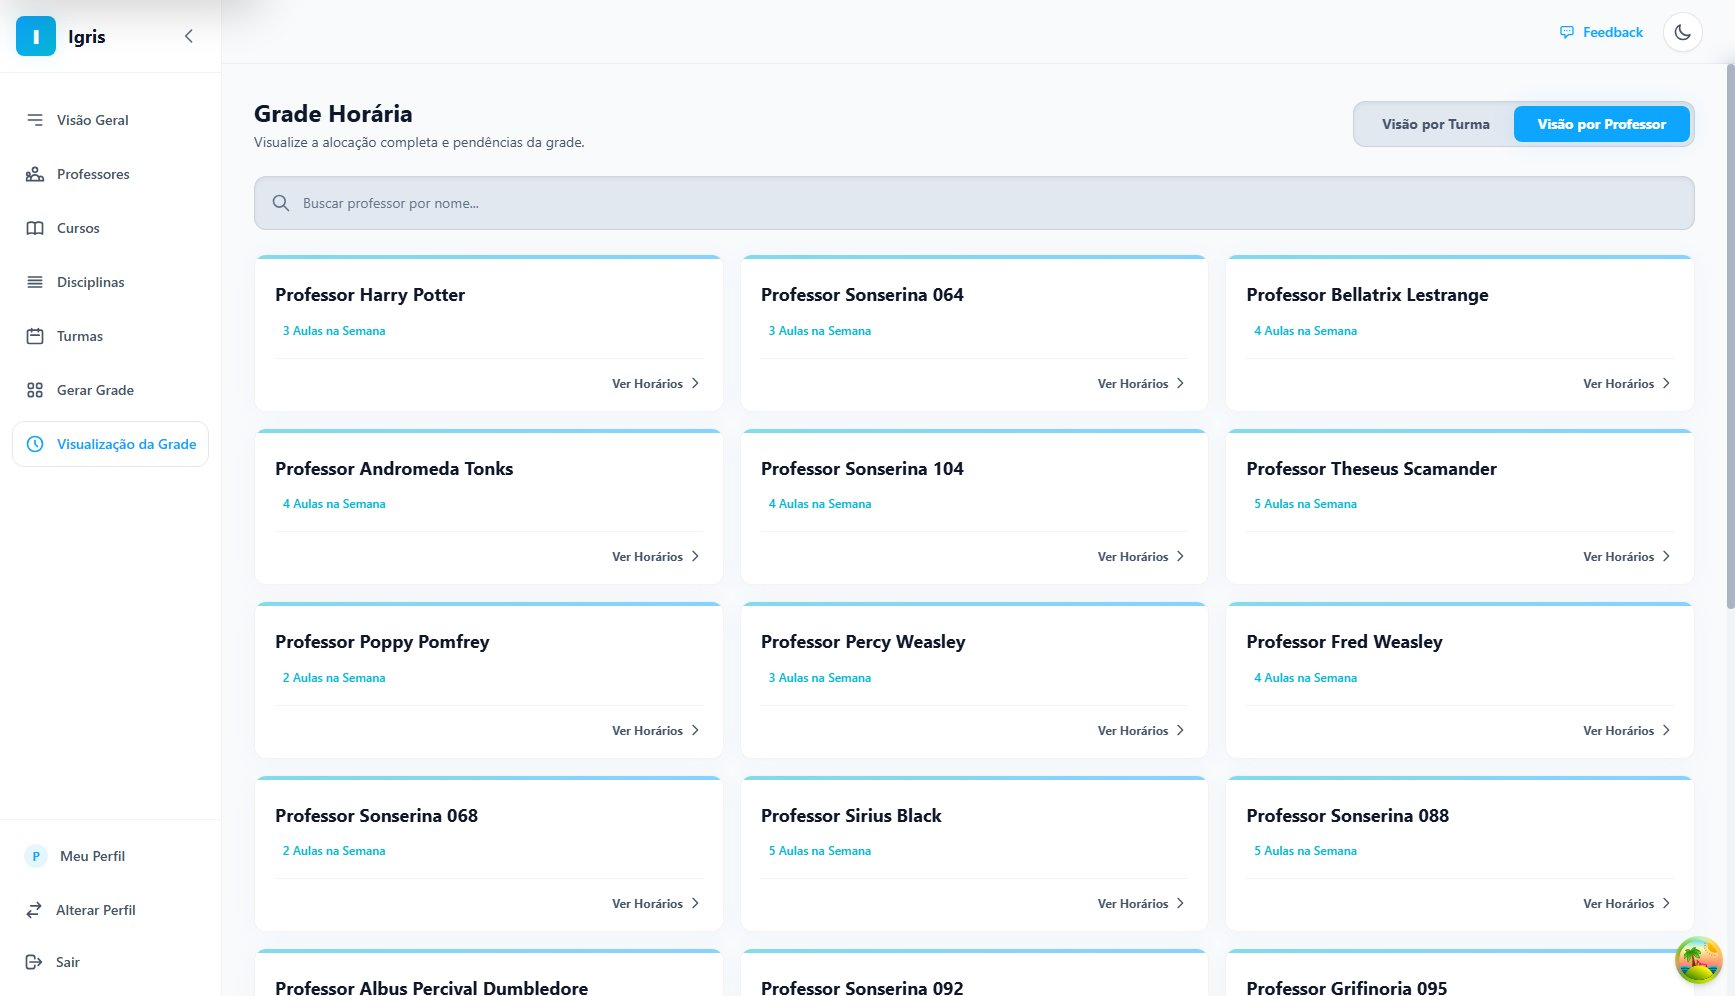
\includegraphics[width=\textwidth]{figuras/paginas/Figura_39_PG24.jpg}
\fonteautores
\end{figure}

A visão por professor organiza a grade horária em cartões individuais para cada docente. Cada cartão apresenta a quantidade de aulas atribuídas na semana e fornece acesso ao detalhamento dos horários, permitindo ao coordenador acompanhar a distribuição da carga docente.

\begin{tabelainteracoes}{Interações da Grade Horária -- Visão por Professor}{tab:interacoes-grade-professor-consulta}
Selecionar ``Visão por Professor'' & O sistema agrupa as aulas da grade ativa por docente. & A quantidade exibida deve considerar somente o período letivo selecionado. \\
\hline
Pesquisar pelo nome do professor & O sistema filtra os cartões conforme o texto informado. & Quando não houver correspondência, deve ser apresentada uma indicação de lista vazia. \\
\hline
Consultar a quantidade de aulas semanais & O sistema apresenta a carga atribuída a cada professor. & O valor auxilia a identificar professores com carga reduzida ou excessiva. \\
\hline
Clicar em ``Ver Horários'' & O sistema abre a matriz semanal do professor selecionado. & O detalhamento deve mostrar apenas as aulas vinculadas ao docente acionado. \\
\hline
Alternar para ``Visão por Turma'' & O sistema reorganiza a mesma grade em cartões de turmas. & A mudança de visualização não modifica as alocações armazenadas. \\
\hline
\end{tabelainteracoes}

% PG25.jpg
\begin{figure}[H]
\centering
\caption{Grade Horária - Detalhamento Semanal do Professor}
\label{fig:PG25}
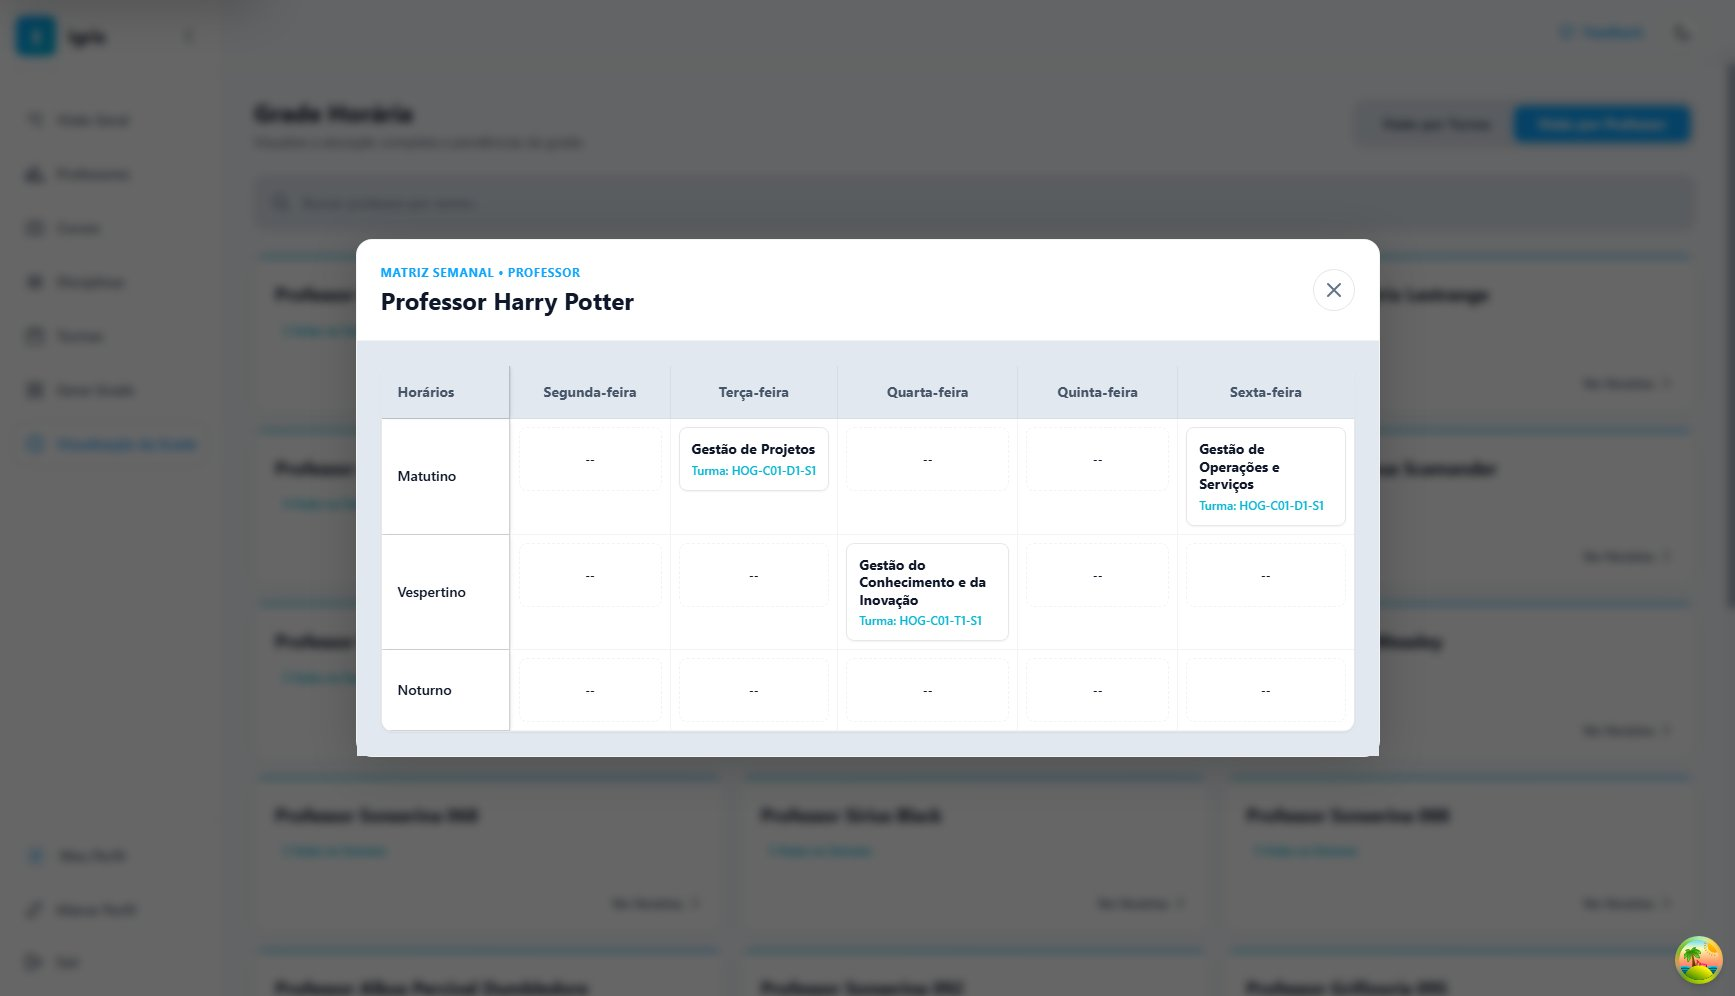
\includegraphics[width=\textwidth]{figuras/paginas/Figura_40_PG25.jpg}
\fonteautores
\end{figure}

A janela apresenta a matriz semanal de um professor selecionado, distribuindo suas aulas entre os dias da semana e os turnos letivos. Cada horário preenchido identifica a disciplina ministrada e a turma correspondente, oferecendo uma visão individual da carga docente.

\begin{tabelainteracoes}{Interações do Detalhamento Semanal do Professor}{tab:interacoes-detalhamento-semanal-professor}
Abrir os horários de um professor & O sistema apresenta a matriz semanal e identifica o docente no cabeçalho. & Os dados devem corresponder à grade ativa e ao período letivo consultado. \\
\hline
Consultar uma célula preenchida & O sistema exibe a disciplina e a turma atribuídas ao professor naquele horário. & A alocação deve respeitar a disponibilidade e as áreas de atuação cadastradas. \\
\hline
Consultar uma célula vazia & O sistema indica que não existe aula atribuída naquele intervalo. & Um período sem aula não representa necessariamente disponibilidade para novas alocações. \\
\hline
Identificar aulas simultâneas & O sistema deve sinalizar a sobreposição para correção. & Um professor não pode ministrar aulas para turmas diferentes no mesmo horário. \\
\hline
Clicar no ícone de fechar & O sistema encerra o detalhamento e retorna à visão por professores. & Fechar a janela não modifica a grade. \\
\hline
\end{tabelainteracoes}

% PG26.jpg
\begin{figure}[H]
\centering
\caption{Painel Acadêmico - Áreas de Atuação do Professor}
\label{fig:PG26}
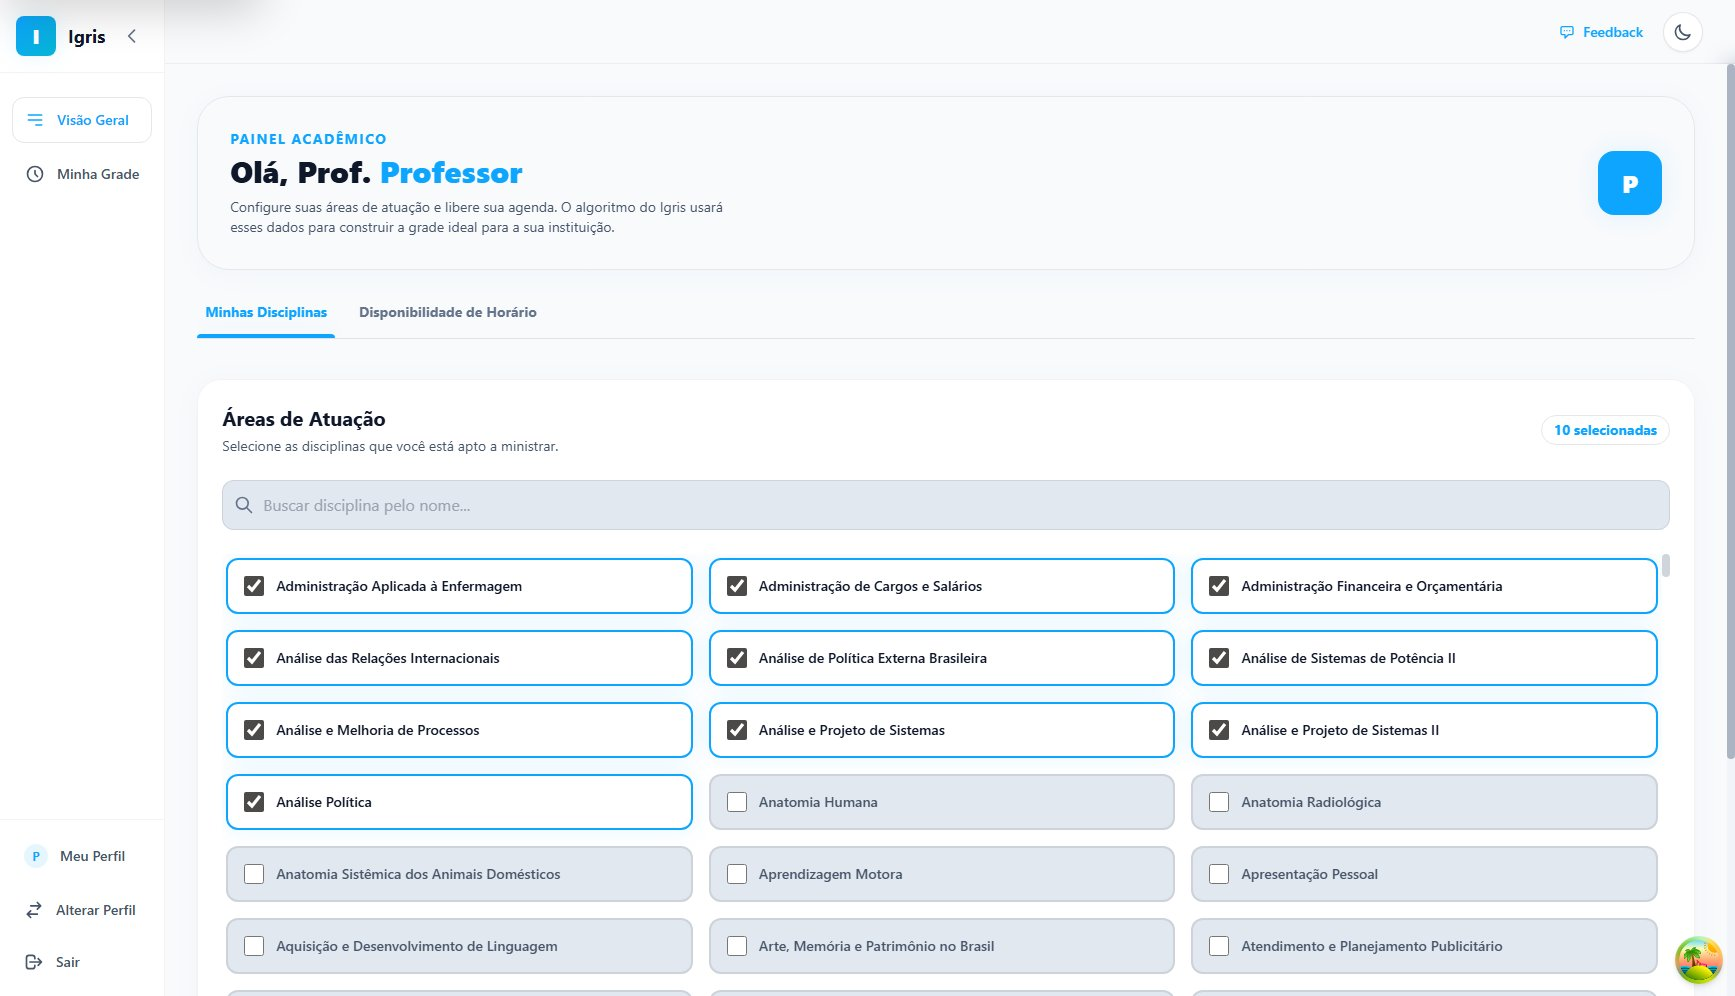
\includegraphics[width=\textwidth]{figuras/paginas/Figura_41_PG26.jpg}
\fonteautores
\end{figure}

No painel acadêmico, a aba ``Minhas Disciplinas'' permite ao professor consultar e selecionar suas áreas de atuação. As disciplinas são apresentadas com caixas de seleção e uma ferramenta de busca, fornecendo ao algoritmo as informações necessárias para realizar alocações compatíveis com a qualificação do docente.

\begin{tabelainteracoes}{Interações das Áreas de Atuação no Painel do Professor}{tab:interacoes-areas-painel-professor}
Selecionar a aba ``Minhas Disciplinas'' & O sistema apresenta as disciplinas disponíveis e destaca aquelas já vinculadas ao professor. & As seleções representam as matérias que o docente está habilitado a ministrar. \\
\hline
Pesquisar uma disciplina & O sistema filtra a relação conforme o termo informado. & As disciplinas selecionadas devem permanecer marcadas mesmo quando não estiverem visíveis no filtro atual. \\
\hline
Marcar uma disciplina & O sistema adiciona a matéria às áreas de atuação do professor. & O vínculo passa a ser considerado pelo algoritmo nas futuras alocações docentes. \\
\hline
Desmarcar uma disciplina & O sistema remove a matéria das áreas de atuação selecionadas. & Se existirem alocações vigentes para a disciplina, o sistema deve alertar sobre o impacto da alteração. \\
\hline
Consultar o total de disciplinas selecionadas & O sistema atualiza o contador apresentado na seção. & O valor facilita a conferência das áreas atualmente associadas ao professor. \\
\hline
Selecionar a aba ``Disponibilidade do Professor'' & O sistema abre o mapa semanal para consulta e manutenção dos horários livres. & As áreas de atuação e a disponibilidade são restrições complementares utilizadas na geração da grade. \\
\hline
\end{tabelainteracoes}

% PG27.jpg
\begin{figure}[H]
\centering
\caption{Áreas de Atuação do Professor}
\label{fig:PG27}
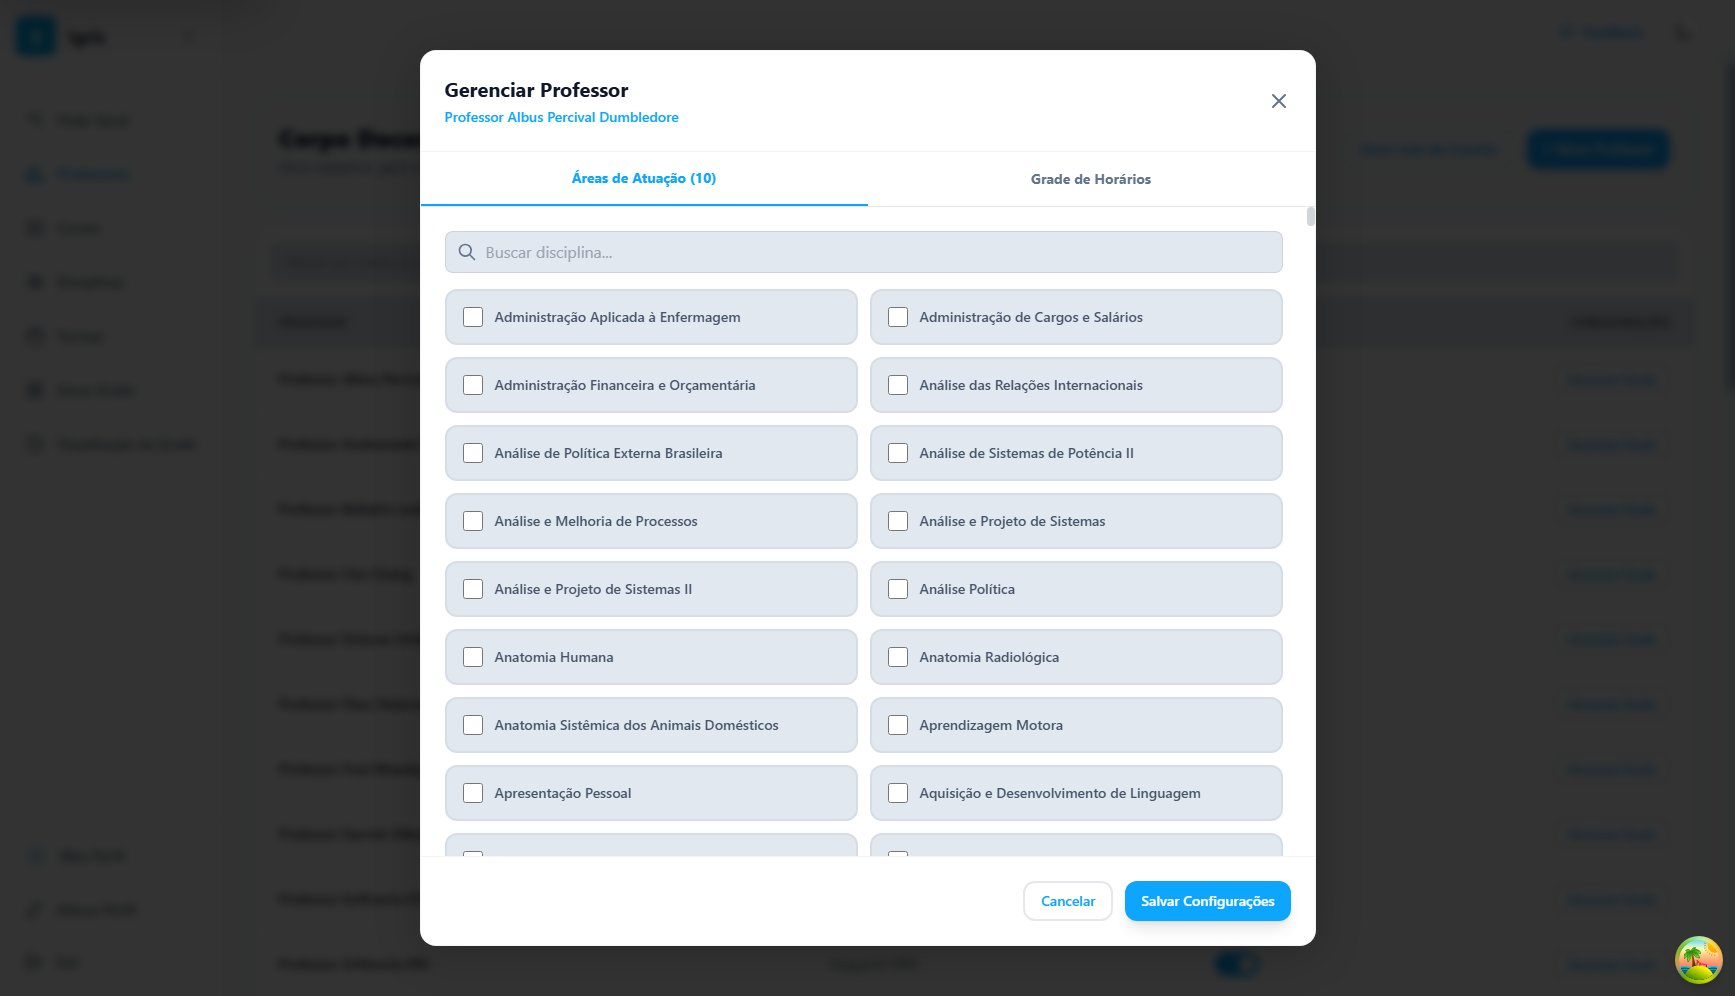
\includegraphics[width=\textwidth]{figuras/paginas/Figura_42_PG27.jpg}
\fonteautores
\end{figure}

O coordenador tem acesso a uma janela de configuração onde define quais disciplinas o professor está habilitado a ministrar, permitindo uma restrição correta baseada nas qualificações.

\begin{tabelainteracoes}{Interações das Áreas de Atuação do Professor}{tab:interacoes-areas-professor}
Pesquisar uma disciplina & O sistema filtra as opções de áreas de atuação disponíveis. & As disciplinas já selecionadas devem permanecer marcadas mesmo quando estiverem fora do filtro atual. \\
\hline
Marcar uma disciplina & O sistema inclui temporariamente a matéria entre as áreas que o professor pode ministrar. & A seleção será considerada como restrição de aptidão nas próximas gerações de grade. \\
\hline
Desmarcar uma disciplina & O sistema remove temporariamente a matéria da lista de habilitações do docente. & Se houver alocações existentes nessa disciplina, o sistema deve alertar sobre o possível impacto. \\
\hline
Clicar em ``Salvar Configurações'' & O sistema persiste os vínculos entre professor e disciplinas e fecha a janela. & A confirmação deve ser exibida e as mudanças devem afetar somente o professor selecionado. \\
\hline
Clicar em ``Cancelar'' ou fechar & O sistema descarta alterações não salvas e retorna à tela anterior. & As áreas previamente armazenadas permanecem inalteradas. \\
\hline
\end{tabelainteracoes}

% PG28.jpg
\begin{figure}[H]
\centering
\caption{Parâmetros do Sistema (Sunny) - Desempenho Rápido}
\label{fig:PG28}
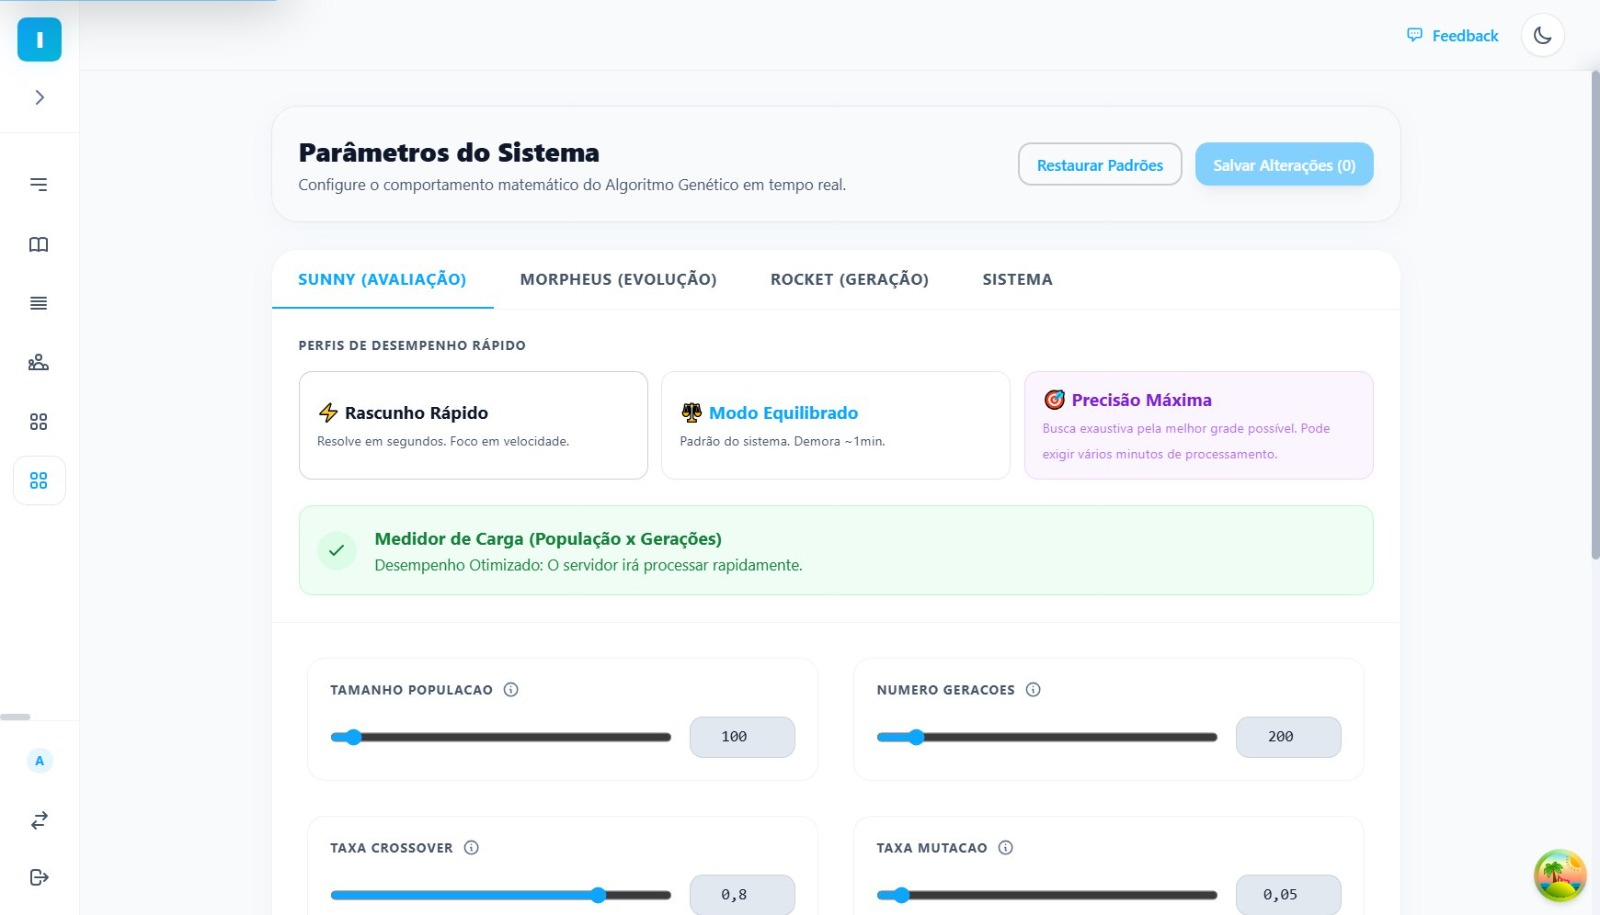
\includegraphics[width=\textwidth]{figuras/paginas/Figura_43_PG28.jpg}
\fonteautores
\end{figure}

A tela oferece perfis de desempenho rápido (Rascunho Rápido, Modo Equilibrado e Modo Perfeição), simplificando a configuração matemática do algoritmo em predefinições.

\begin{tabelainteracoes}{Interações dos Parâmetros do Sistema -- Desempenho Rápido}{tab:interacoes-perfis-desempenho}
Selecionar ``Rascunho Rápido'' & O sistema aplica parâmetros voltados à obtenção de resultado em menor tempo. & A execução tende a consumir menos recursos, podendo produzir uma solução com qualidade inferior. \\
\hline
Selecionar ``Modo Equilibrado'' & O sistema aplica uma combinação intermediária entre tempo de processamento e qualidade. & É a opção recomendada para uso geral quando não há necessidade de ajuste manual. \\
\hline
Selecionar ``Modo Perfeição'' & O sistema aplica parâmetros mais intensivos para ampliar a busca por uma solução de maior qualidade. & O modo pode aumentar significativamente o tempo e o consumo computacional. \\
\hline
Alterar manualmente um parâmetro após escolher um perfil & O sistema atualiza o valor e passa a tratar a configuração como personalizada. & O medidor de carga deve ser recalculado imediatamente. \\
\hline
Clicar em ``Salvar Alterações'' & O sistema persiste o perfil e os valores apresentados para futuras execuções. & A configuração não deve modificar resultados ou grades já armazenados. \\
\hline
Clicar em ``Restaurar Padrões'' & O sistema repõe a predefinição padrão do algoritmo selecionado. & Uma confirmação evita a perda acidental de ajustes personalizados. \\
\hline
\end{tabelainteracoes}

% PG29.jpg
\begin{figure}[H]
\centering
\caption{Auditoria do Corpo de Coordenadores}
\label{fig:PG29}
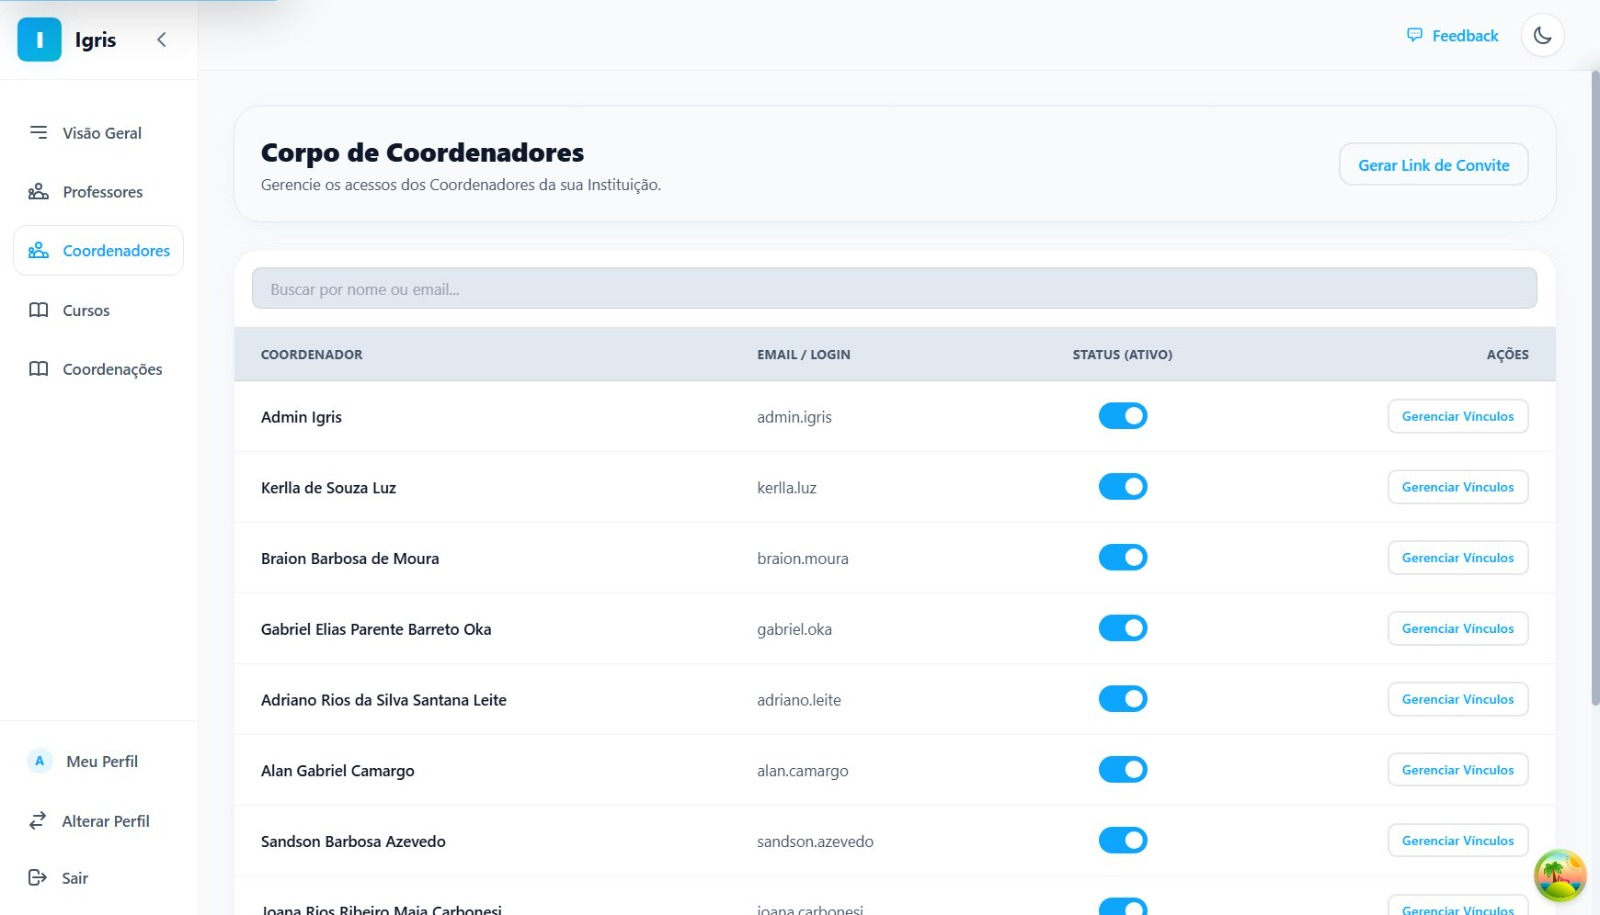
\includegraphics[width=\textwidth]{figuras/paginas/Figura_44_PG29.jpg}
\fonteautores
\end{figure}

Os acessos do quadro gestor institucional podem ser auditados e controlados através desta listagem centralizada, que promove transparência na gestão.

\begin{tabelainteracoes}{Interações da Auditoria do Corpo de Coordenadores}{tab:interacoes-auditoria-coordenadores}
Pesquisar um coordenador & O sistema filtra a lista pelo nome ou e-mail do gestor. & A consulta deve permanecer limitada à instituição administrada pelo usuário. \\
\hline
Consultar o status de acesso & O sistema apresenta se o perfil do coordenador está ativo ou inativo. & O status exibido deve refletir o valor atualmente persistido. \\
\hline
Ativar ou desativar um coordenador & O sistema atualiza a permissão de acesso e registra a alteração. & A auditoria deve preservar autor, data e estado alterado quando o sistema possuir histórico de ações. \\
\hline
Clicar em ``Ver Configuração'' & O sistema apresenta os perfis e coordenações associados ao usuário. & O administrador pode verificar se os privilégios concedidos são compatíveis com a função exercida. \\
\hline
Gerar um link de convite & O sistema cria um convite para inclusão de um novo gestor. & O ingresso do usuário deve permanecer sujeito às regras de validação e atribuição de coordenação. \\
\hline
\end{tabelainteracoes}

% PG30.jpg
\begin{figure}[H]
\centering
\caption{Adição e Atribuição de Coordenações}
\label{fig:PG30}
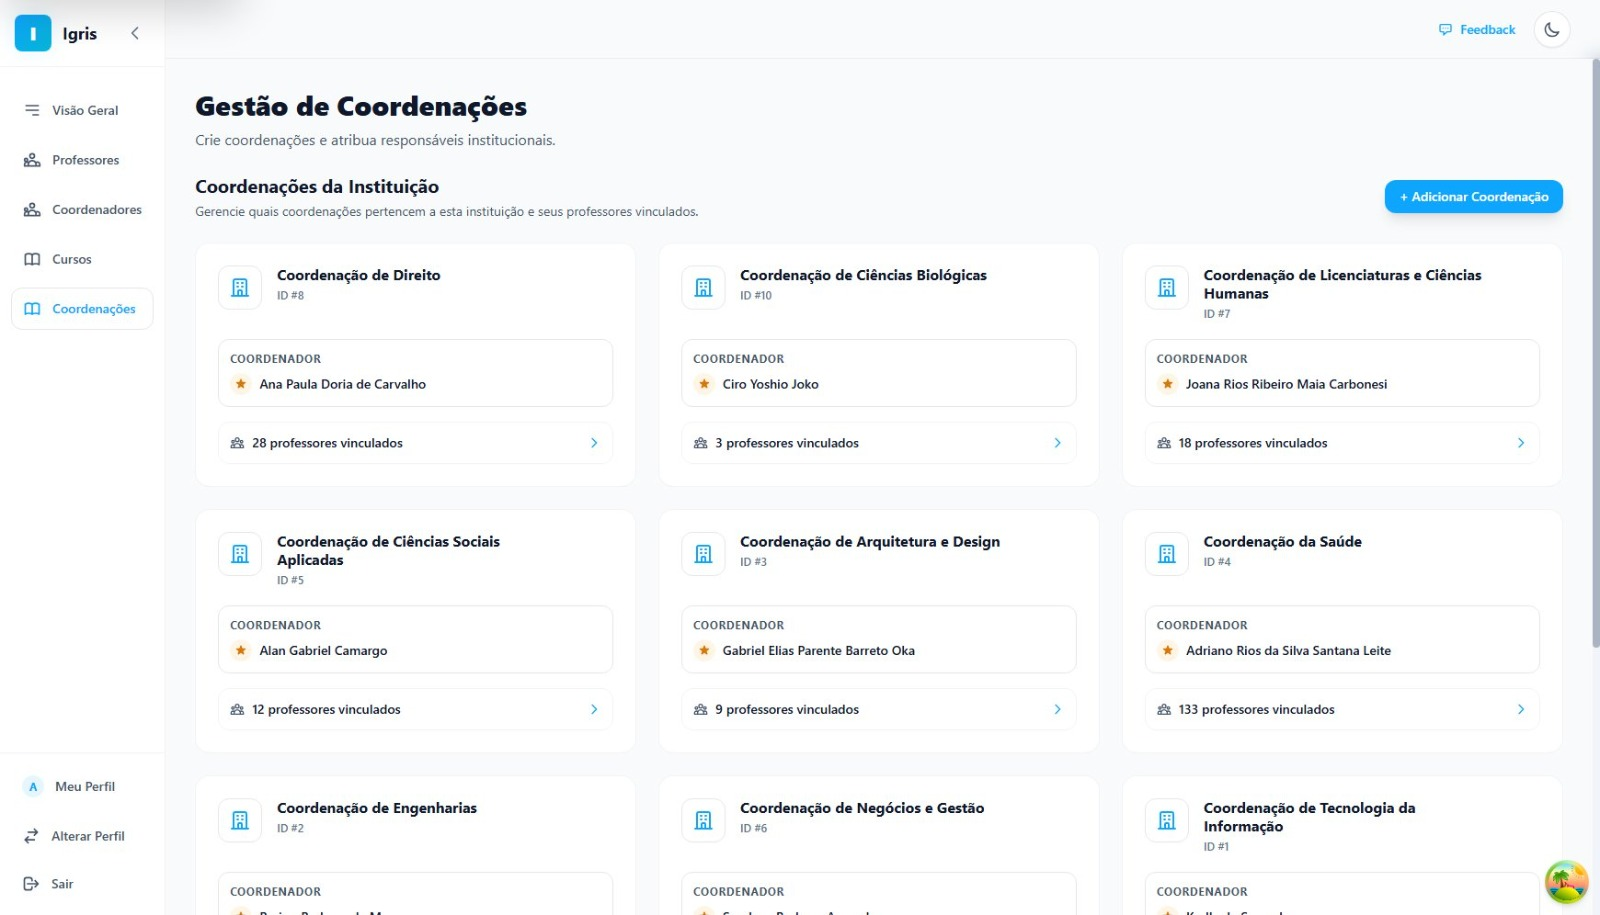
\includegraphics[width=\textwidth]{figuras/paginas/Figura_45_PG30.jpg}
\fonteautores
\end{figure}

A interface evidencia que os responsáveis podem ser rapidamente identificados e que novas áreas podem ser estruturadas com agilidade.

\begin{tabelainteracoes}{Interações da Adição e Atribuição de Coordenações}{tab:interacoes-adicao-coordenacoes}
Informar o nome da nova coordenação & O sistema prepara o cadastro de uma nova área institucional. & O nome deve ser obrigatório e não pode duplicar outra coordenação da mesma instituição. \\
\hline
Clicar em ``Adicionar'' & O sistema cria a coordenação e a inclui na tabela. & Uma mensagem deve confirmar a operação ou explicar a falha de validação. \\
\hline
Consultar os responsáveis de uma coordenação & O sistema apresenta os coordenadores atualmente vinculados à área. & A ausência de responsáveis deve ser sinalizada para evitar uma coordenação sem gestão definida. \\
\hline
Selecionar um coordenador para atribuição & O sistema cria o vínculo entre o usuário, seu perfil e a coordenação escolhida. & O usuário precisa possuir um cadastro válido e permissão compatível. \\
\hline
Remover um responsável & O sistema solicita confirmação e encerra o vínculo com a coordenação. & A remoção não exclui o usuário; se for o único responsável, o sistema deve alertar sobre a área ficar sem coordenador. \\
\hline
\end{tabelainteracoes}

% PG31.jpg
\begin{figure}[H]
\centering
\caption{Indicadores de Carga do Sistema e Algoritmo}
\label{fig:PG31}
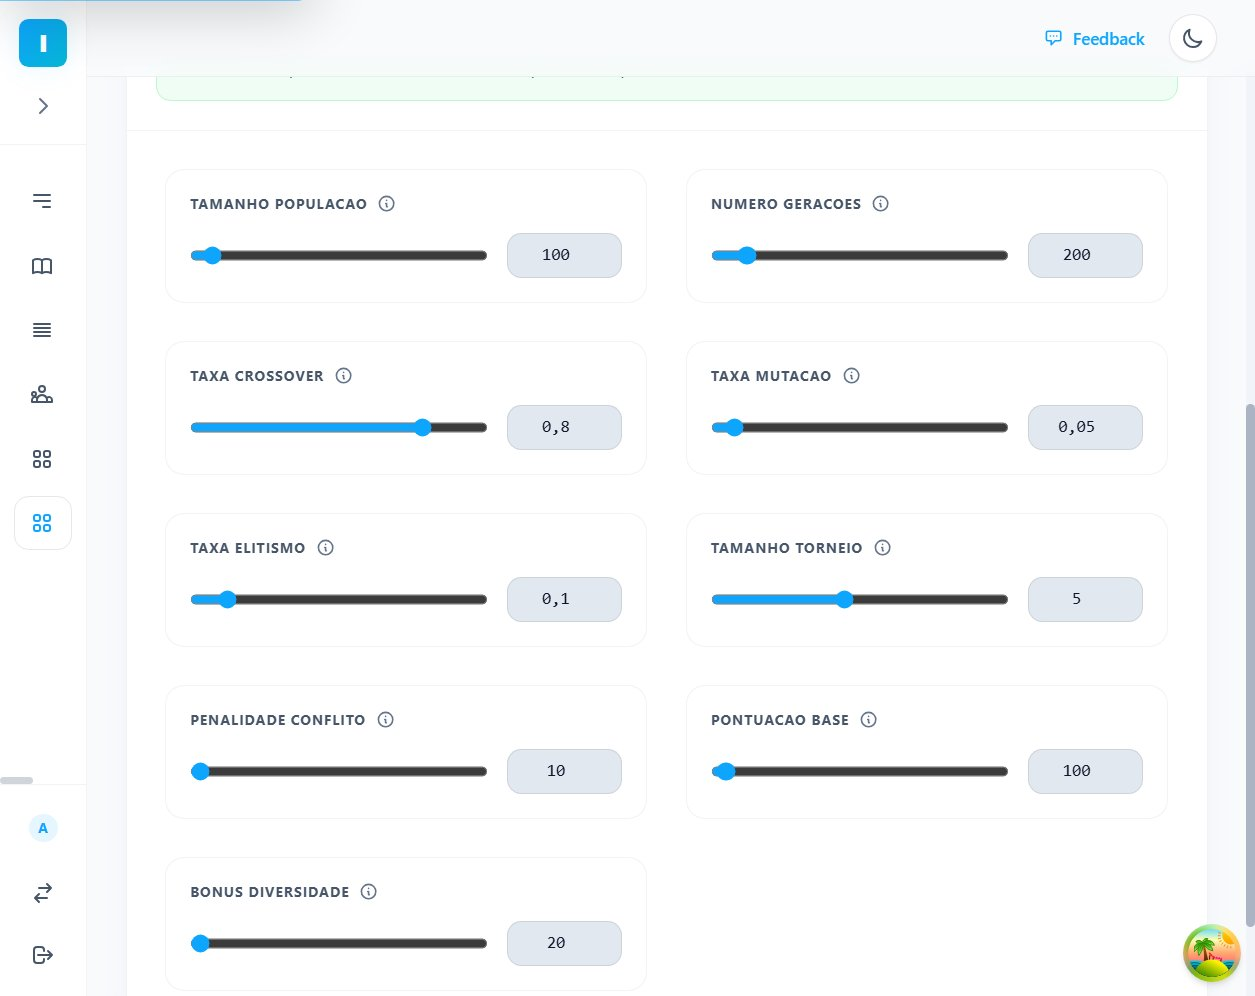
\includegraphics[width=\textwidth]{figuras/paginas/Figura_46_PG31.jpg}
\fonteautores
\end{figure}

O Medidor de Carga ajuda o gestor a equilibrar a eficiência do processamento algorítmico de forma que as interações funcionem sem sobrecarregar a infraestrutura da nuvem.

\begin{tabelainteracoes}{Interações dos Indicadores de Carga do Sistema e Algoritmo}{tab:interacoes-indicadores-carga}
Mover os controles de população ou gerações & O sistema atualiza os valores e recalcula a carga estimada da execução. & Aumentar esses parâmetros amplia o espaço de busca e normalmente eleva o tempo de processamento. \\
\hline
Ajustar taxas evolutivas e penalidades & O sistema atualiza a configuração matemática do algoritmo. & Cada controle deve respeitar sua faixa válida e exibir o valor exato aplicado. \\
\hline
Consultar o indicador superior & O sistema apresenta uma avaliação textual e visual da configuração atual. & A cor e a mensagem devem permitir reconhecer rapidamente uma carga segura ou elevada. \\
\hline
Definir valores potencialmente excessivos & O sistema alerta sobre risco de demora ou sobrecarga antes do salvamento ou da execução. & Limites críticos podem ser bloqueados conforme a capacidade da infraestrutura. \\
\hline
Salvar os parâmetros & O sistema persiste a configuração para as próximas gerações de grade. & O salvamento deve invalidar configurações em cache para que os motores recebam os novos valores. \\
\hline
\end{tabelainteracoes}

% PG32.jpg
\begin{figure}[H]
\centering
\caption{Disponibilidade Semanal do Professor pelo Coordenador}
\label{fig:PG32}
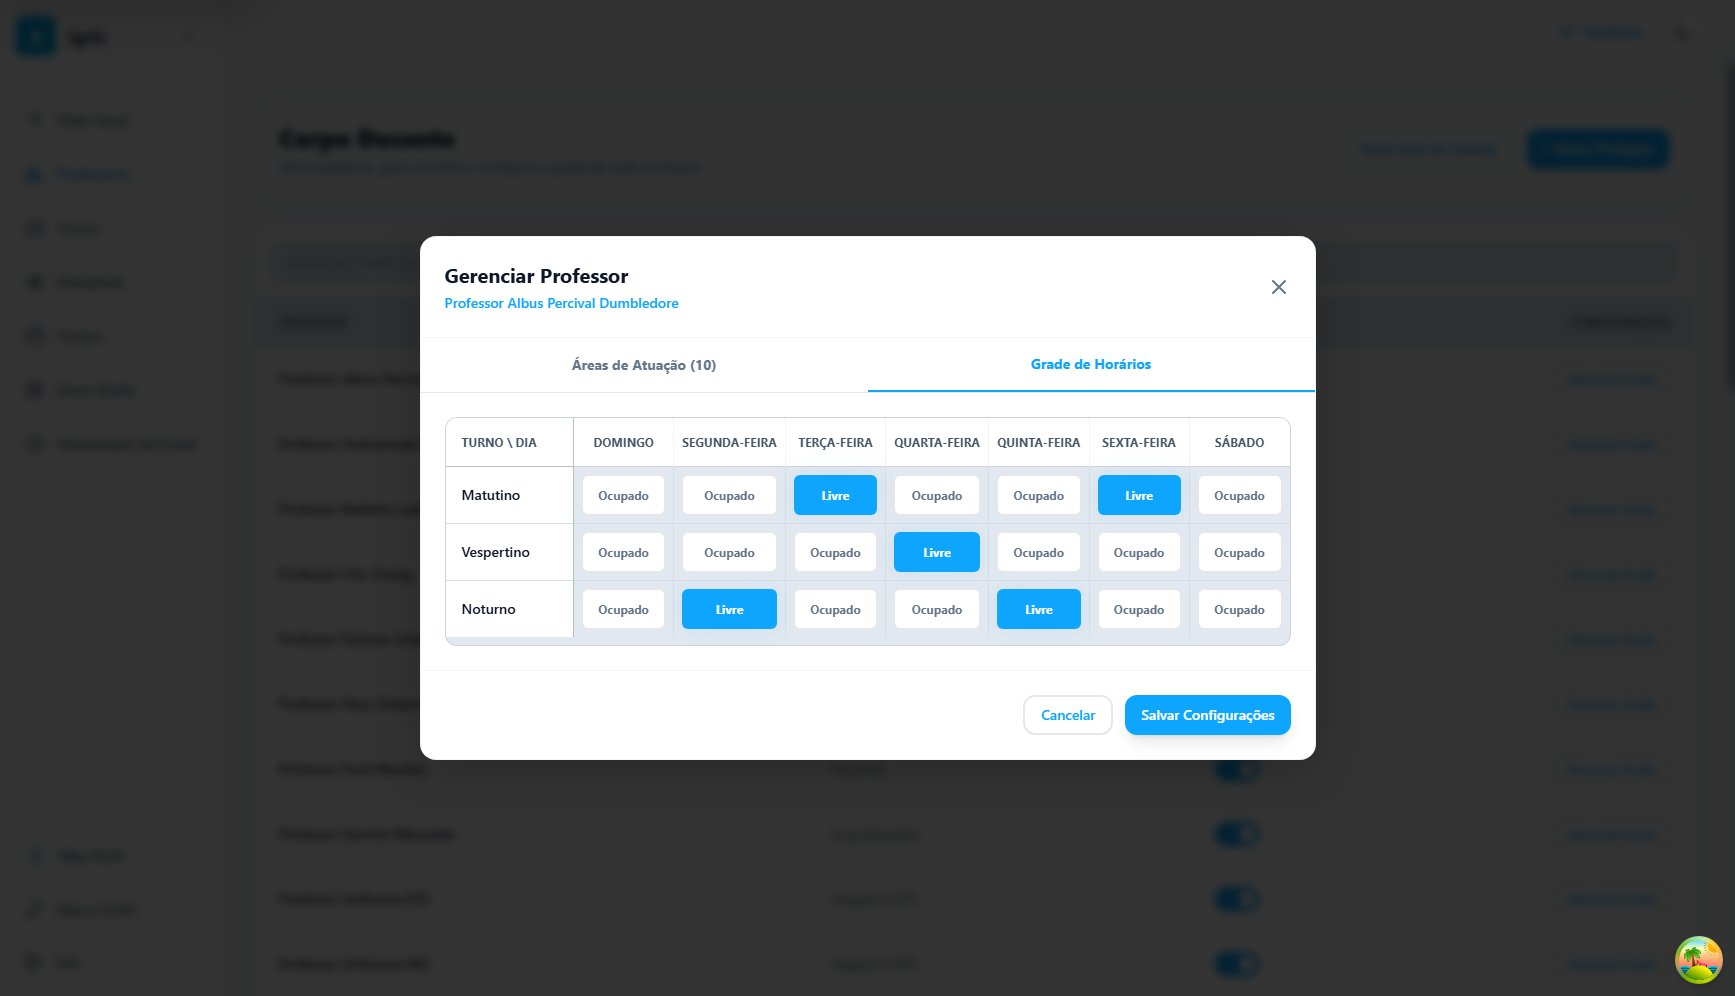
\includegraphics[width=\textwidth]{figuras/paginas/Figura_47_PG32.jpg}
\fonteautores
\end{figure}

A aba Grade de Horários permite ao coordenador visualizar e estabelecer as restrições semanais de disponibilidade de um docente, separadas por dias e turnos.

\begin{tabelainteracoes}{Interações da Disponibilidade Semanal do Professor pelo Coordenador}{tab:interacoes-disponibilidade-coordenador}
Selecionar a aba ``Grade de Horários'' & O sistema apresenta a disponibilidade semanal do professor em uma matriz de dias e turnos. & A janela deve manter a identificação do docente selecionado. \\
\hline
Clicar em um horário ocupado ou indisponível & O sistema alterna o período para livre, quando a alteração for permitida. & A representação visual deve distinguir claramente os estados ``Livre'' e ``Ocupado''. \\
\hline
Clicar em um horário livre & O sistema alterna o período para ocupado ou indisponível. & A mudança é temporária até que as configurações sejam salvas. \\
\hline
Clicar em ``Salvar Configurações'' & O sistema valida e persiste a disponibilidade do professor. & Duplicidades devem ser evitadas e alterações que afetem uma grade já ativa podem exigir alerta. \\
\hline
Clicar em ``Cancelar'' ou fechar & O sistema descarta as mudanças não salvas e retorna ao gerenciamento docente. & A disponibilidade anteriormente registrada permanece inalterada. \\
\hline
\end{tabelainteracoes}

% PG33.jpg
\begin{figure}[H]
\centering
\caption{Painel Acadêmico - Mapa de Disponibilidade do Professor}
\label{fig:PG33}
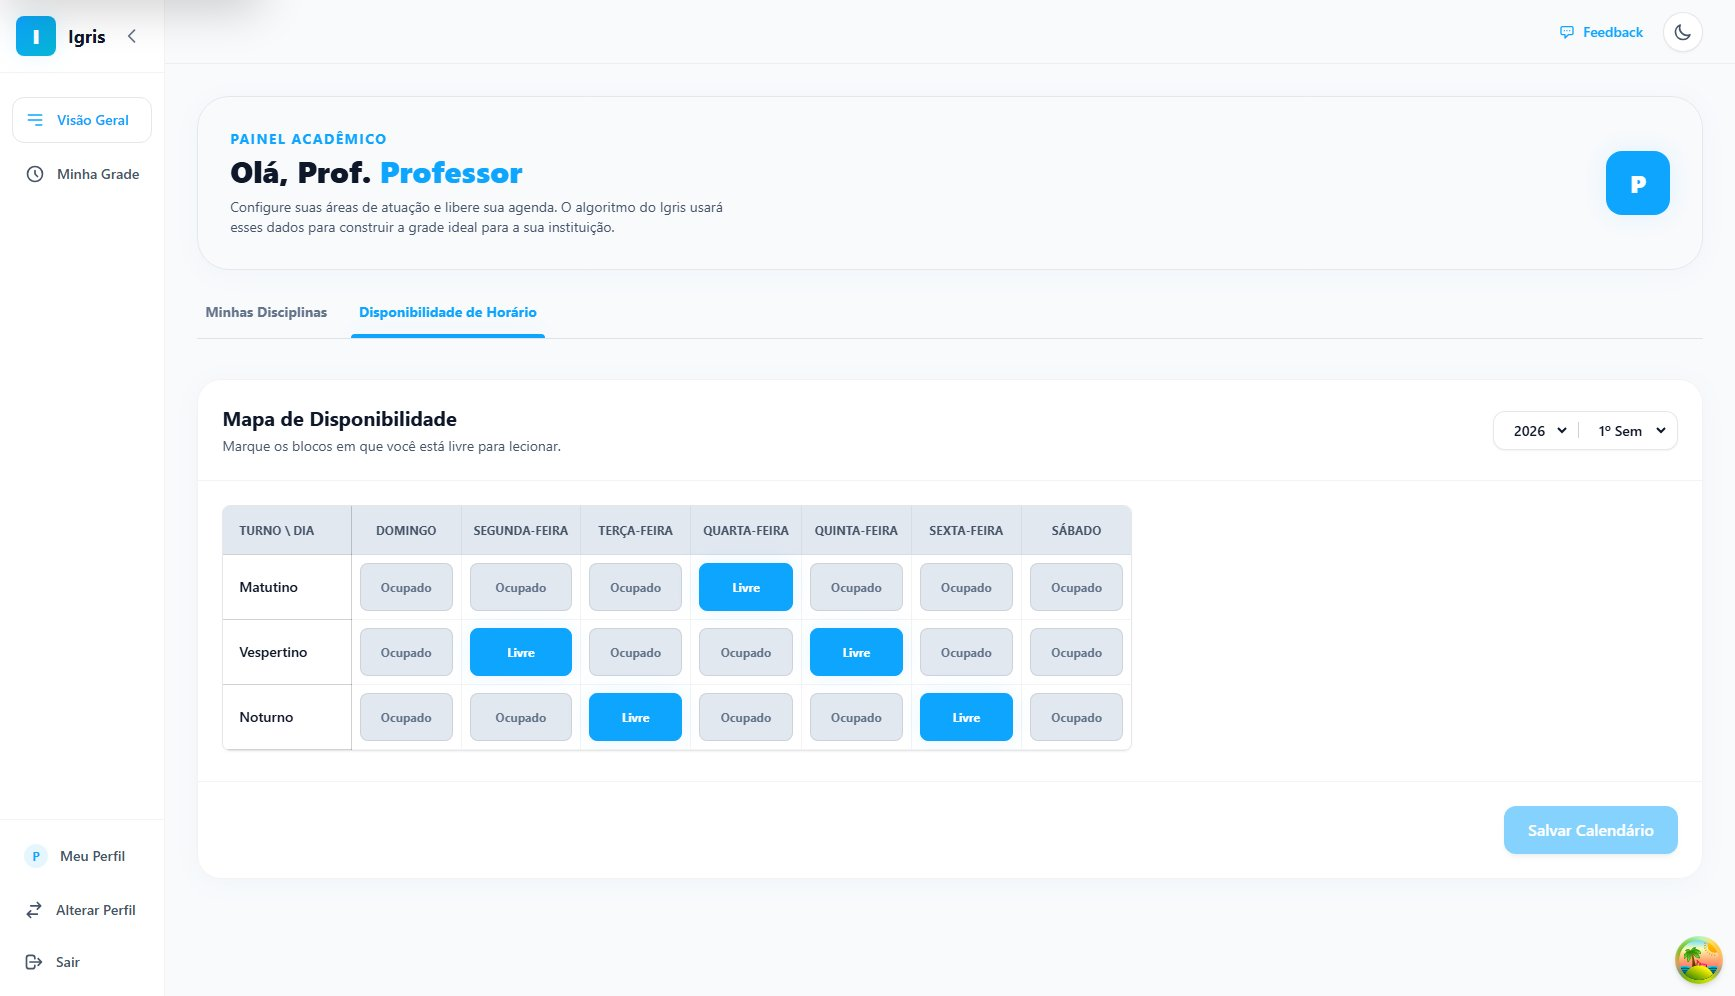
\includegraphics[width=\textwidth]{figuras/paginas/Figura_48_PG33.jpg}
\fonteautores
\end{figure}

No acesso exclusivo do professor, o Mapa de Disponibilidade e a seleção das Áreas de Atuação são centralizados, permitindo que o docente preencha sua matriz semanal autonomamente.

\begin{tabelainteracoes}{Interações do Painel Acadêmico -- Mapa de Disponibilidade do Professor}{tab:interacoes-mapa-disponibilidade-professor}
Selecionar ano e semestre & O sistema carrega a disponibilidade correspondente ao período letivo escolhido. & A manutenção deve ocorrer separadamente para cada combinação de ano e semestre. \\
\hline
Clicar em um bloco da matriz semanal & O sistema alterna o estado do horário entre livre e ocupado. & O estado visual deve ser atualizado imediatamente, mas a alteração só se torna definitiva após o salvamento. \\
\hline
Clicar em ``Salvar Calendário'' & O sistema verifica duplicidades e persiste a disponibilidade informada pelo professor. & Uma mensagem deve confirmar o salvamento; falhas devem manter os dados na tela para nova tentativa. \\
\hline
Trocar de período com alterações não salvas & O sistema alerta sobre a possível perda das modificações antes de carregar outro calendário. & O usuário deve poder cancelar a troca e salvar os dados atuais. \\
\hline
Selecionar a aba ``Minhas Disciplinas'' & O sistema apresenta as áreas de atuação vinculadas ao professor. & A lista permite consultar as disciplinas consideradas pelo algoritmo nas alocações docentes. \\
\hline
Não existir configuração para o período & O sistema apresenta a matriz inicial vazia ou padrão para preenchimento. & Nenhum horário deve ser considerado disponível sem confirmação do professor, conforme a regra institucional. \\
\hline
\end{tabelainteracoes}
